\documentclass[10pt]{beamer}
 
\usepackage[T1]{fontenc}
\usepackage[utf8]{inputenc}
\usepackage{graphicx}
\usepackage{hyperref}
\usepackage{lmodern}
\usepackage{listings}
\usepackage{amssymb} 
\usepackage{xcolor}
\usetheme{Warsaw}
\usepackage{tikz}
\setbeamercovered{transparent}

\author{Latrille Thibault, Nicolas Lartillot, Laurent Duret}
\title{The red queen dynamic in the kingdom of recombination.}  
\institute{Laboratoire de Biométrie et Biologie Évolutive (LBBE), UMR CNRS 5558, Lyon}

\sloppy 

 
\begin{document}

\frame{\titlepage} 

\begin{frame}
	\begin{center}
       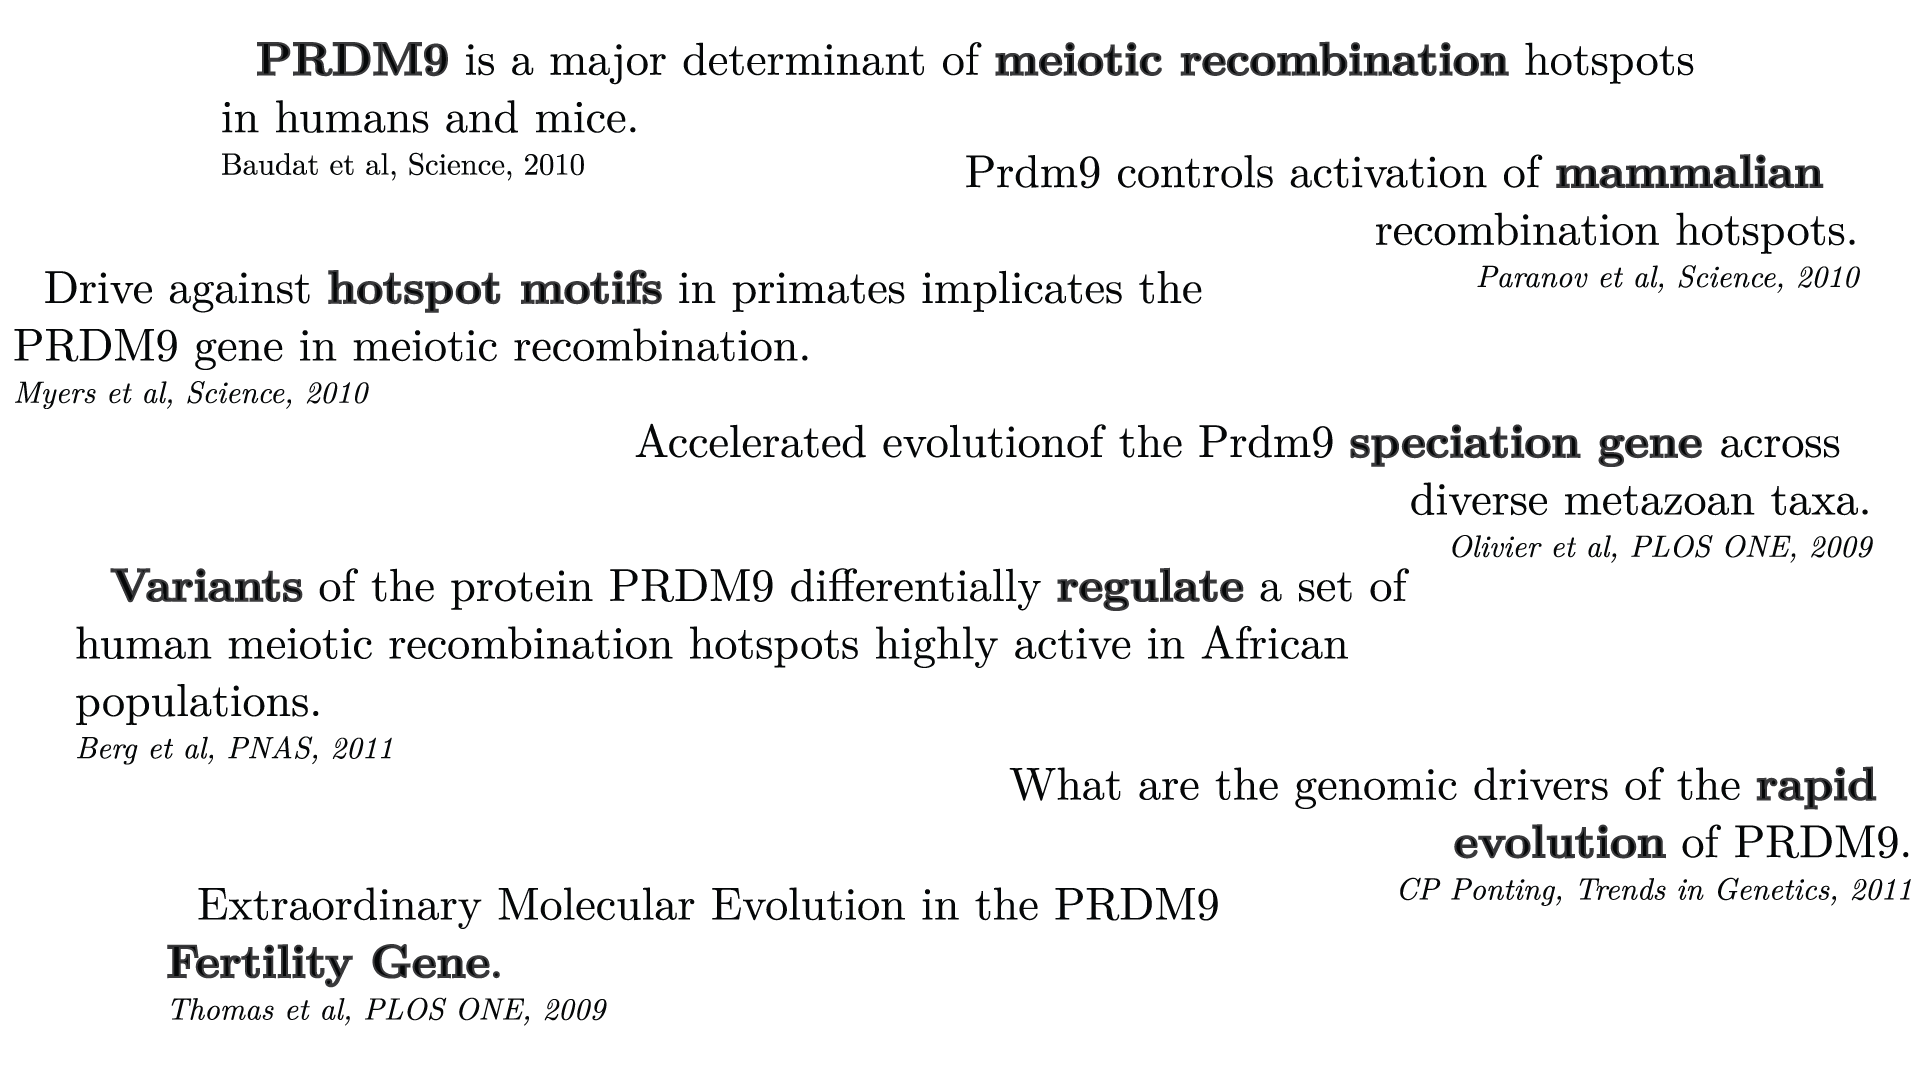
\includegraphics[width=11cm]{Images/publications.png}
	\end{center}
\end{frame}

\begin{frame}
\frametitle{Overline of the presentation}
	\begin{center}
       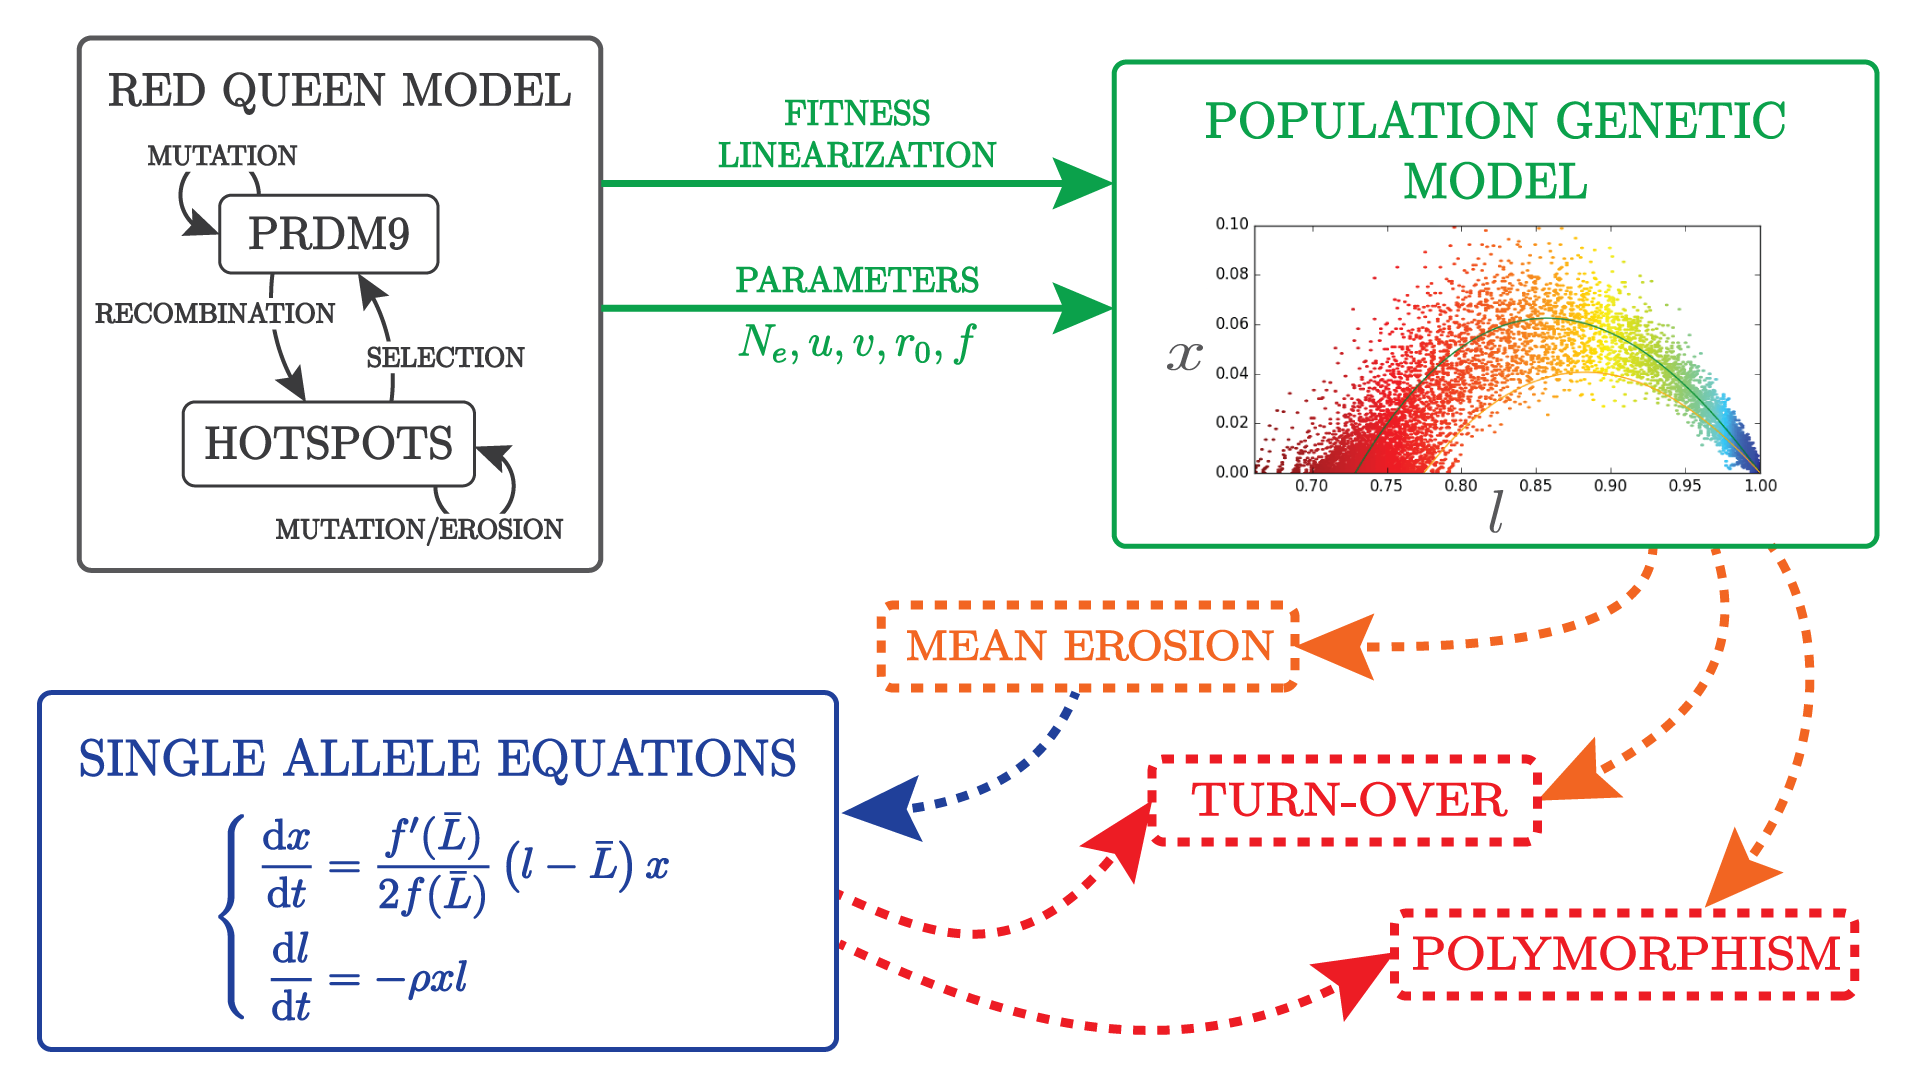
\includegraphics[width=8.5cm]{Images/overline.png}
	\end{center}
\end{frame}

\section{Red queen model}

\begin{frame}
	\begin{center}
	\huge
	Chapter 1. \\
       Red queen model
	\end{center}
\end{frame}

\begin{frame}
	\begin{center}
       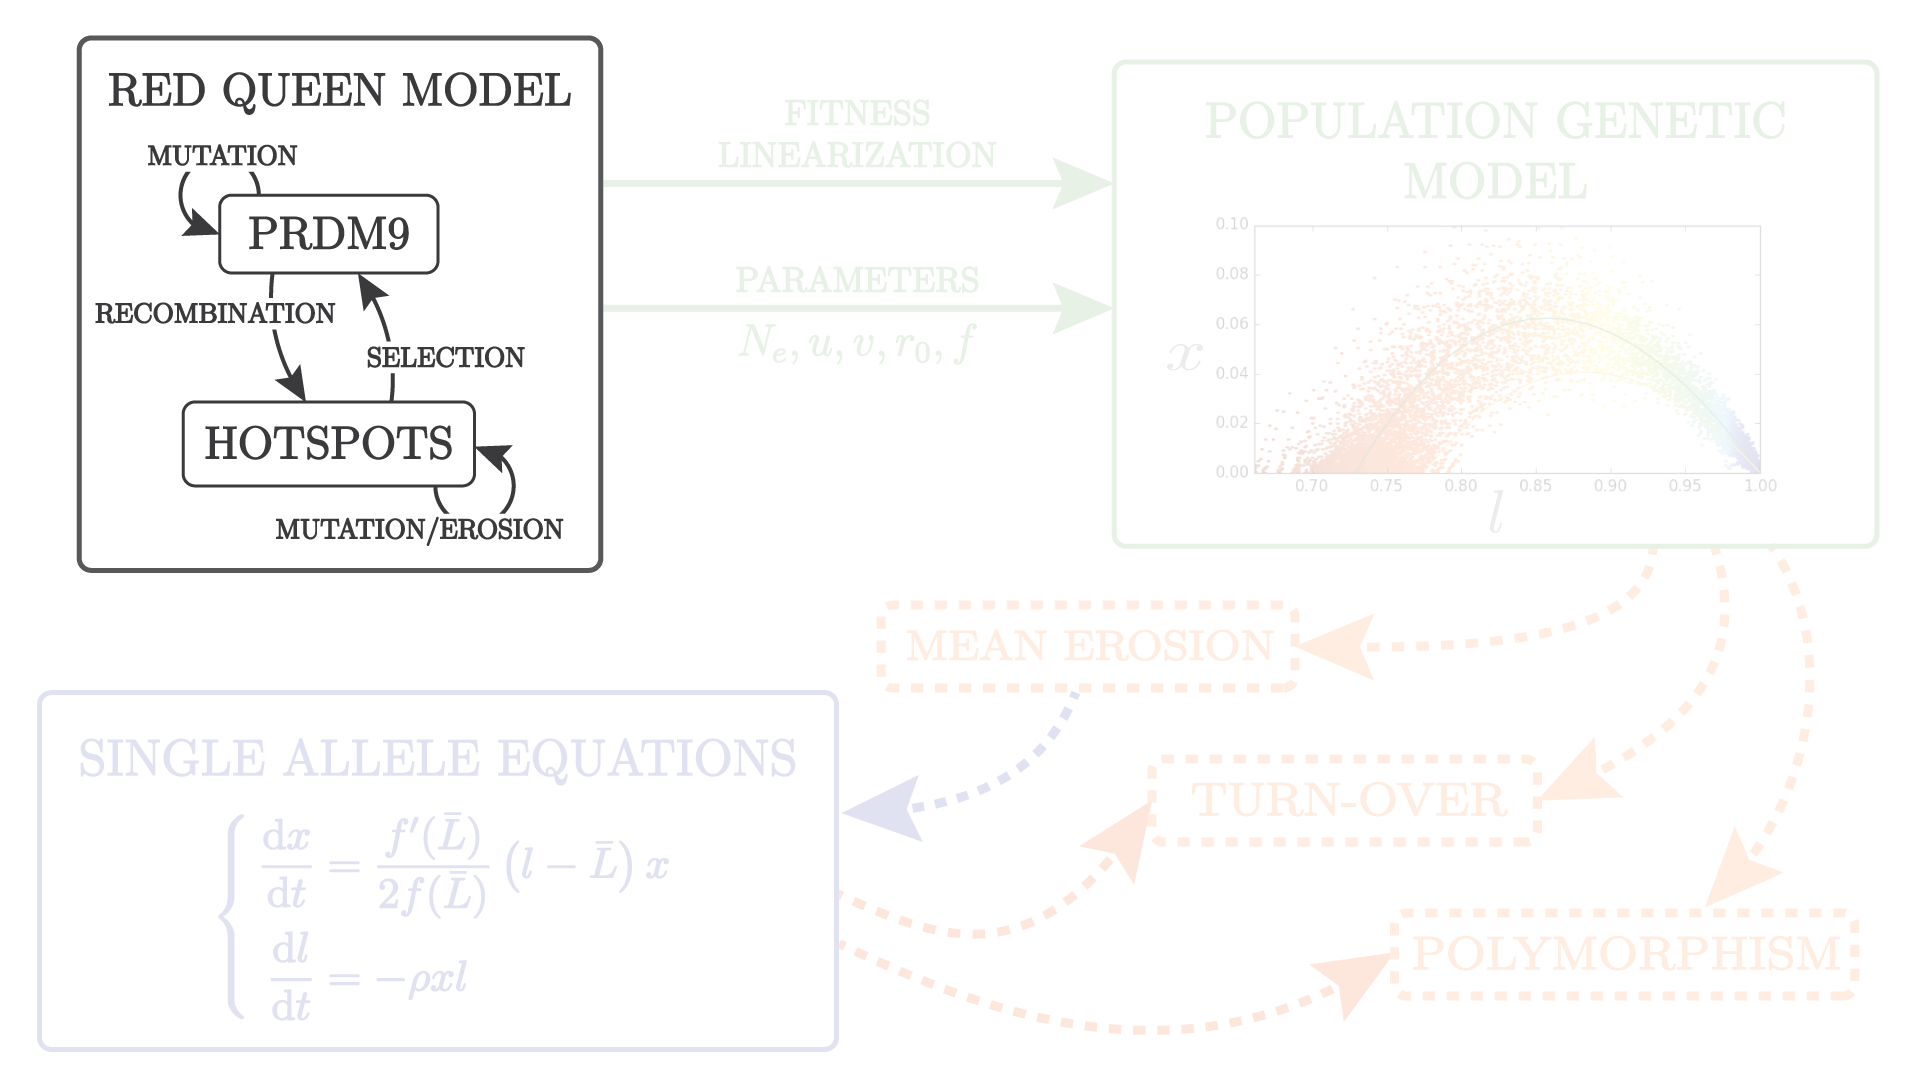
\includegraphics[width=8.5cm]{Images/overline-1.png}
	\end{center}
\end{frame}

\begin{frame}
\frametitle{Recombination of the hotspots ruled by PRDM9}
	\begin{center}
       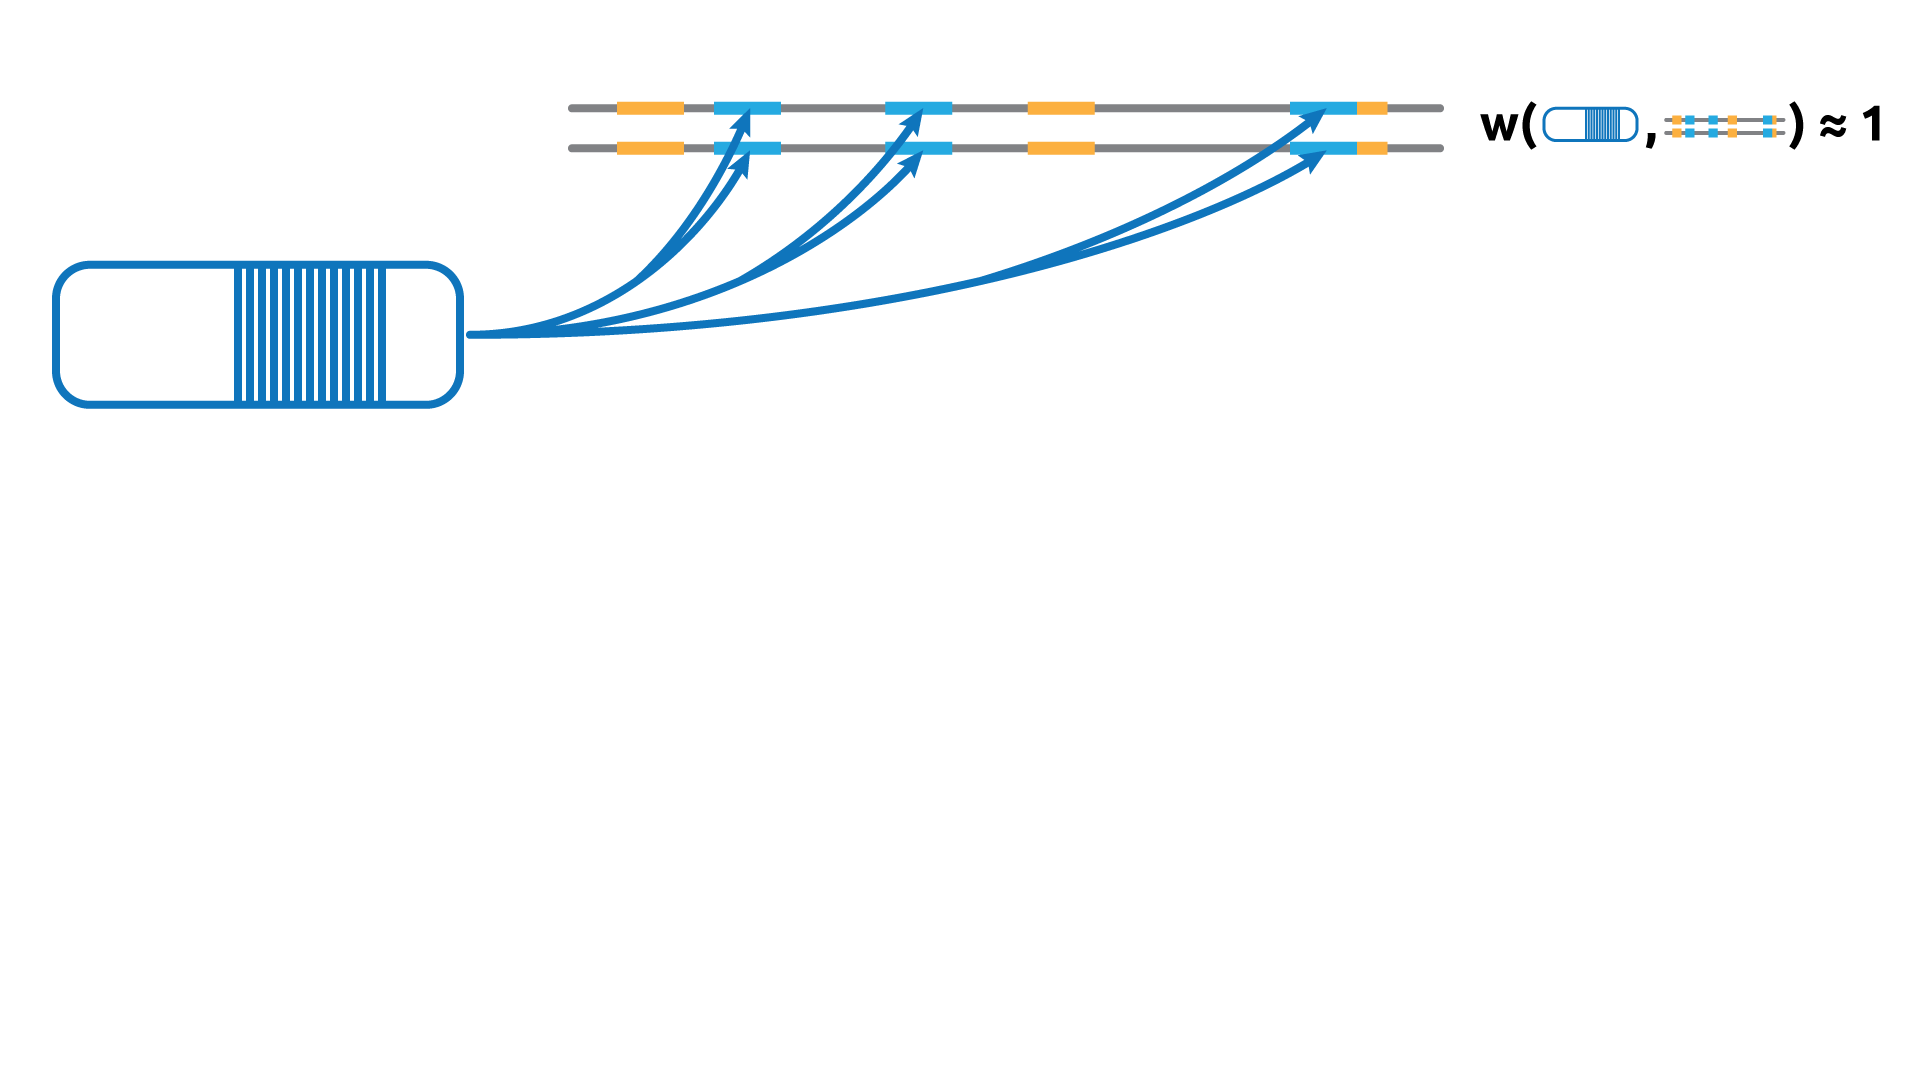
\includegraphics[width=9cm]{Images/red-queen-1.png}
	\end{center}
\end{frame}

\begin{frame}
\frametitle{Erosion of the hotspots and selection of PRDM9}
	\begin{center}
       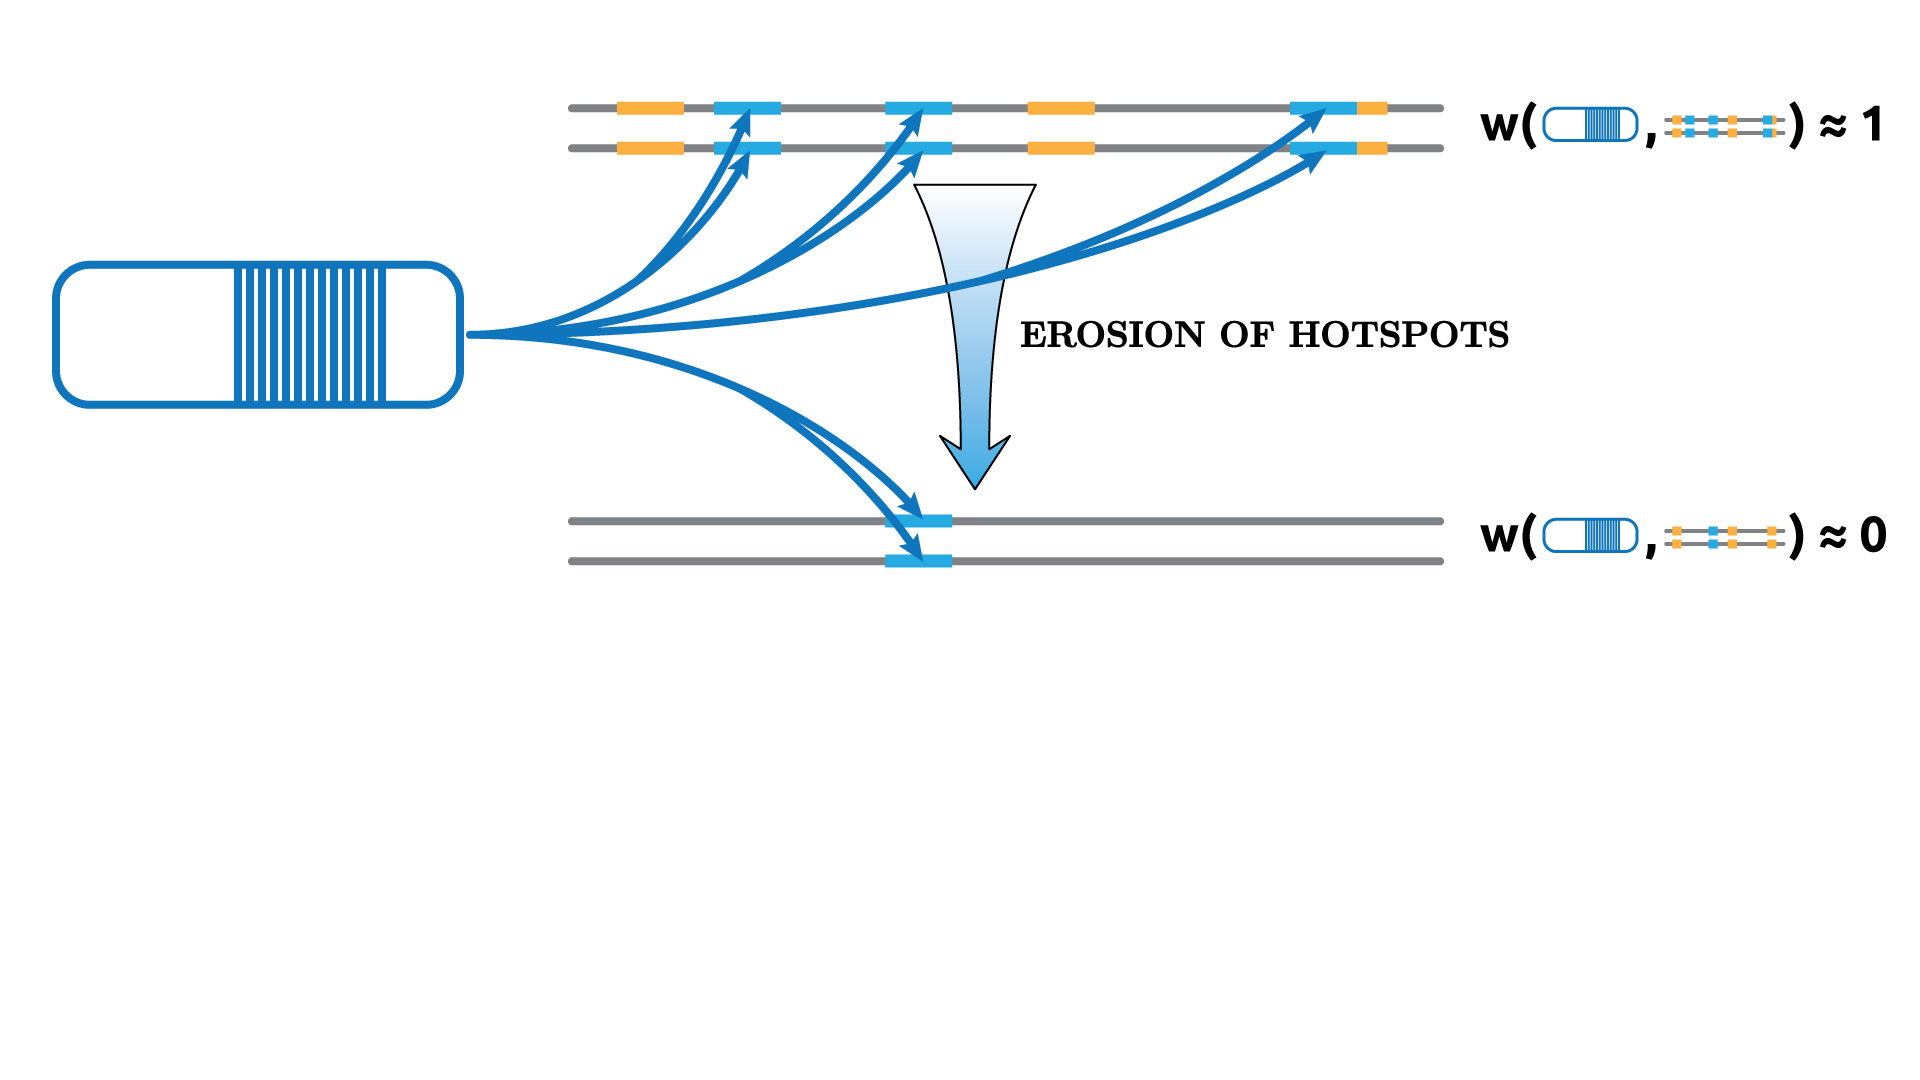
\includegraphics[width=9cm]{Images/red-queen-2.png}
	\end{center}
\end{frame}

\begin{frame}
\frametitle{Mutation of PRDM9}
	\begin{center}
       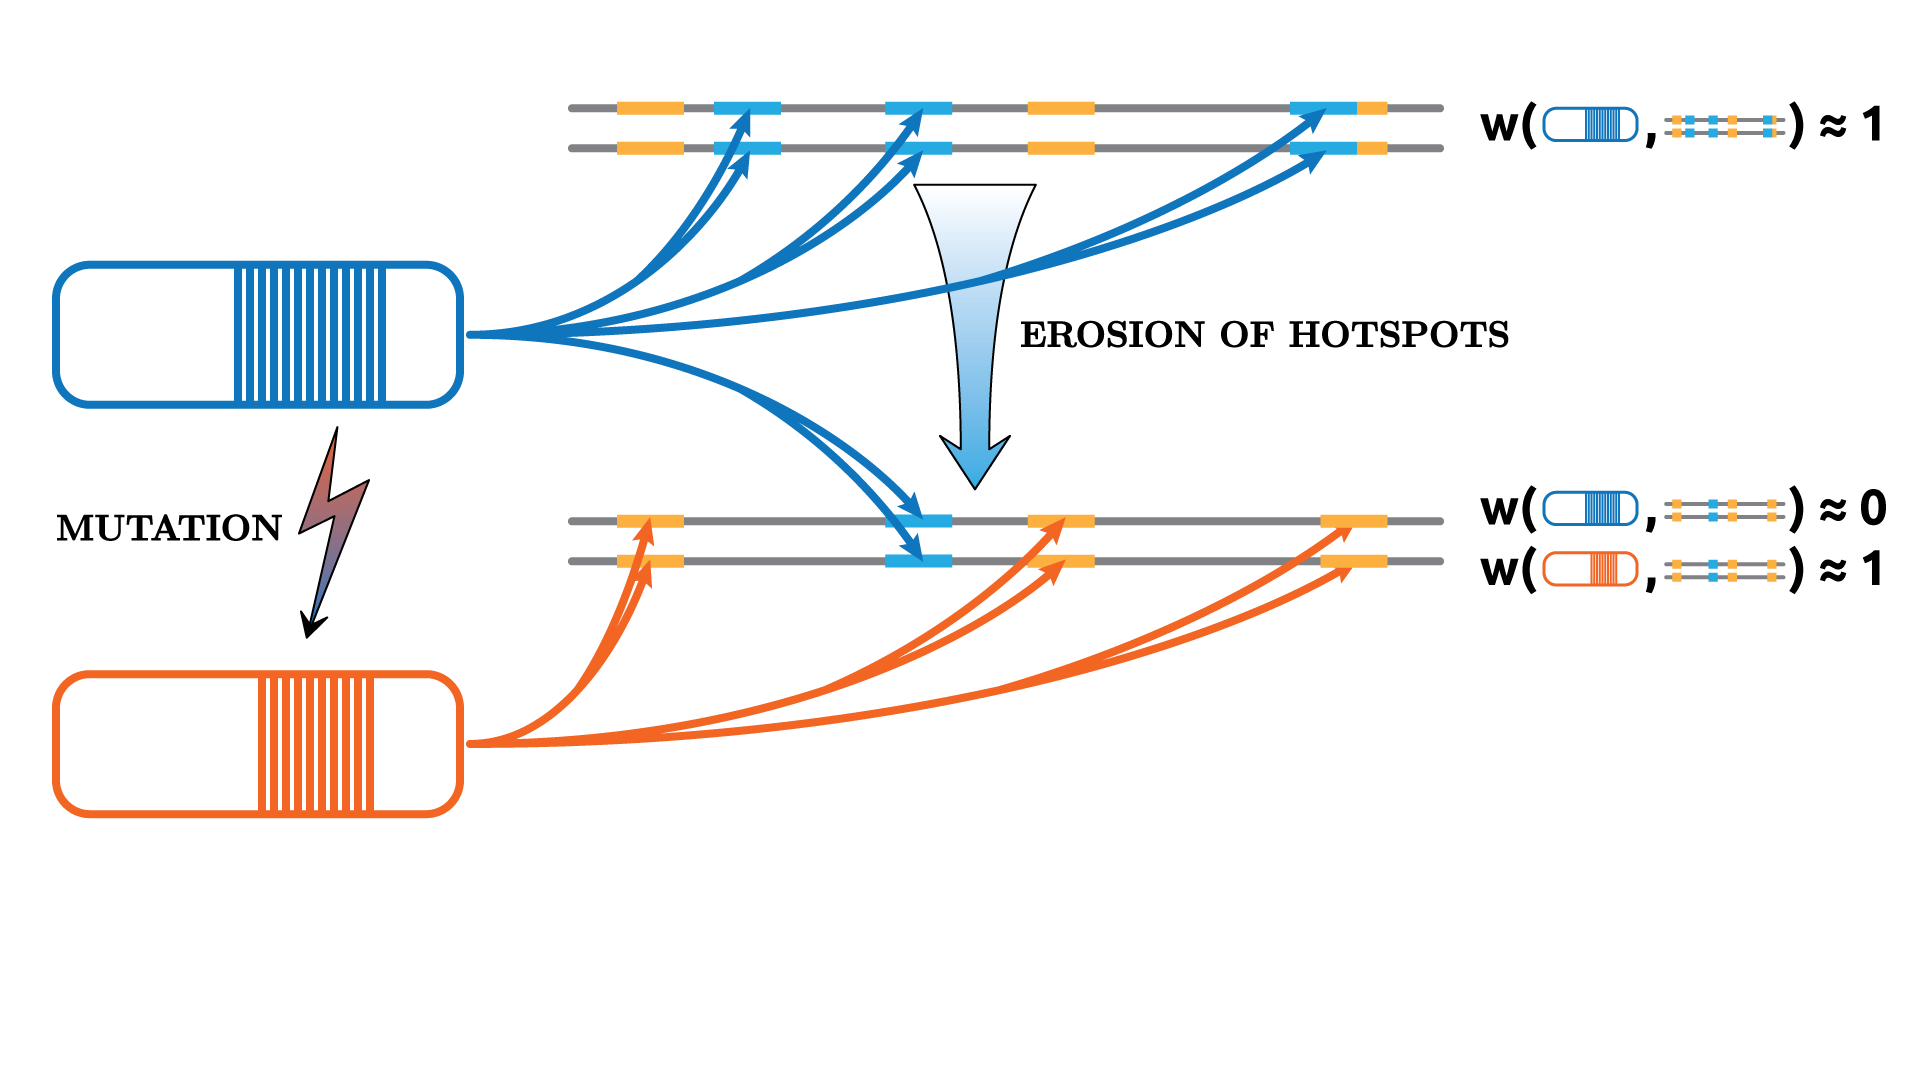
\includegraphics[width=9cm]{Images/red-queen-4.png}
	\end{center}
\end{frame}

\begin{frame}
\frametitle{Erosion, again and again...}
	\begin{center}
       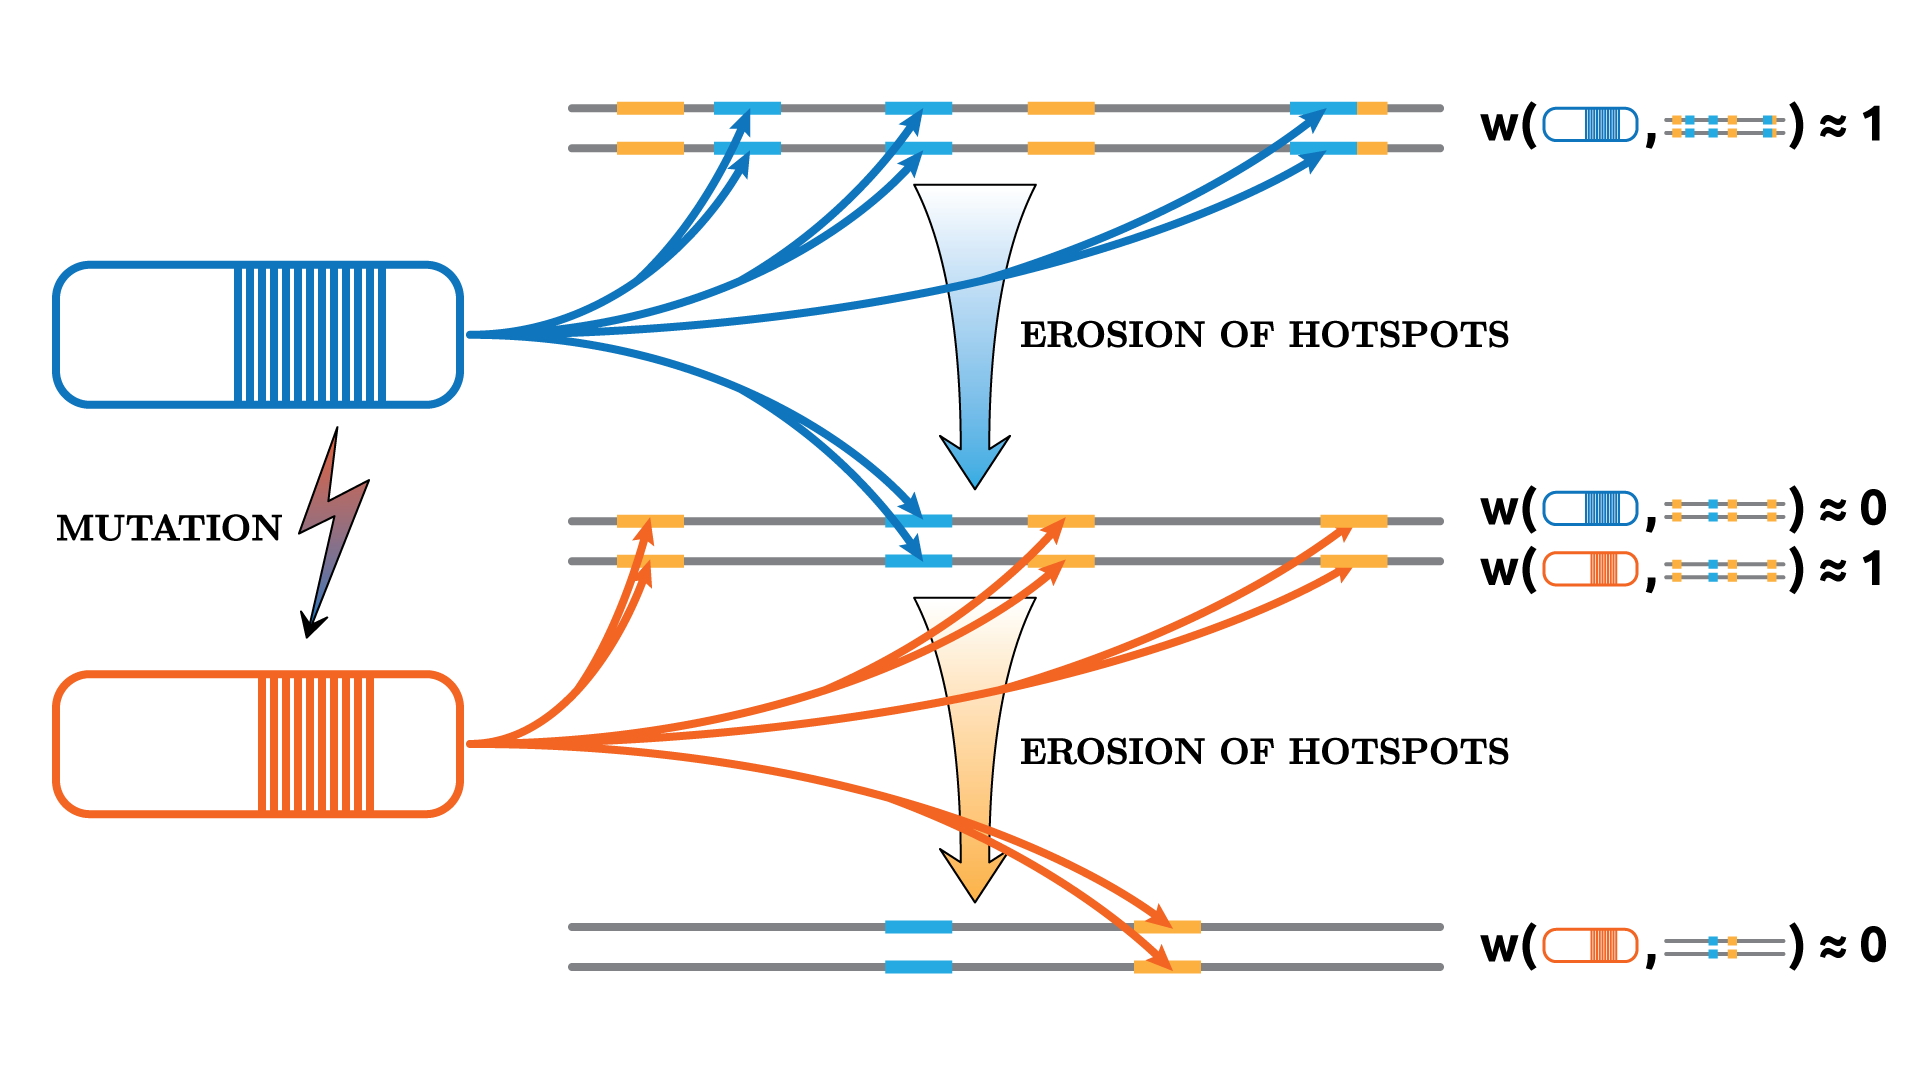
\includegraphics[width=9cm]{Images/red-queen-5.png}
	\end{center}
\end{frame}

\section{Population genetic model}

\begin{frame}
	\begin{center}
	\huge
	Chapter 2. \\
       Population genetic model
	\end{center}
\end{frame}

\begin{frame}
	\begin{center}
       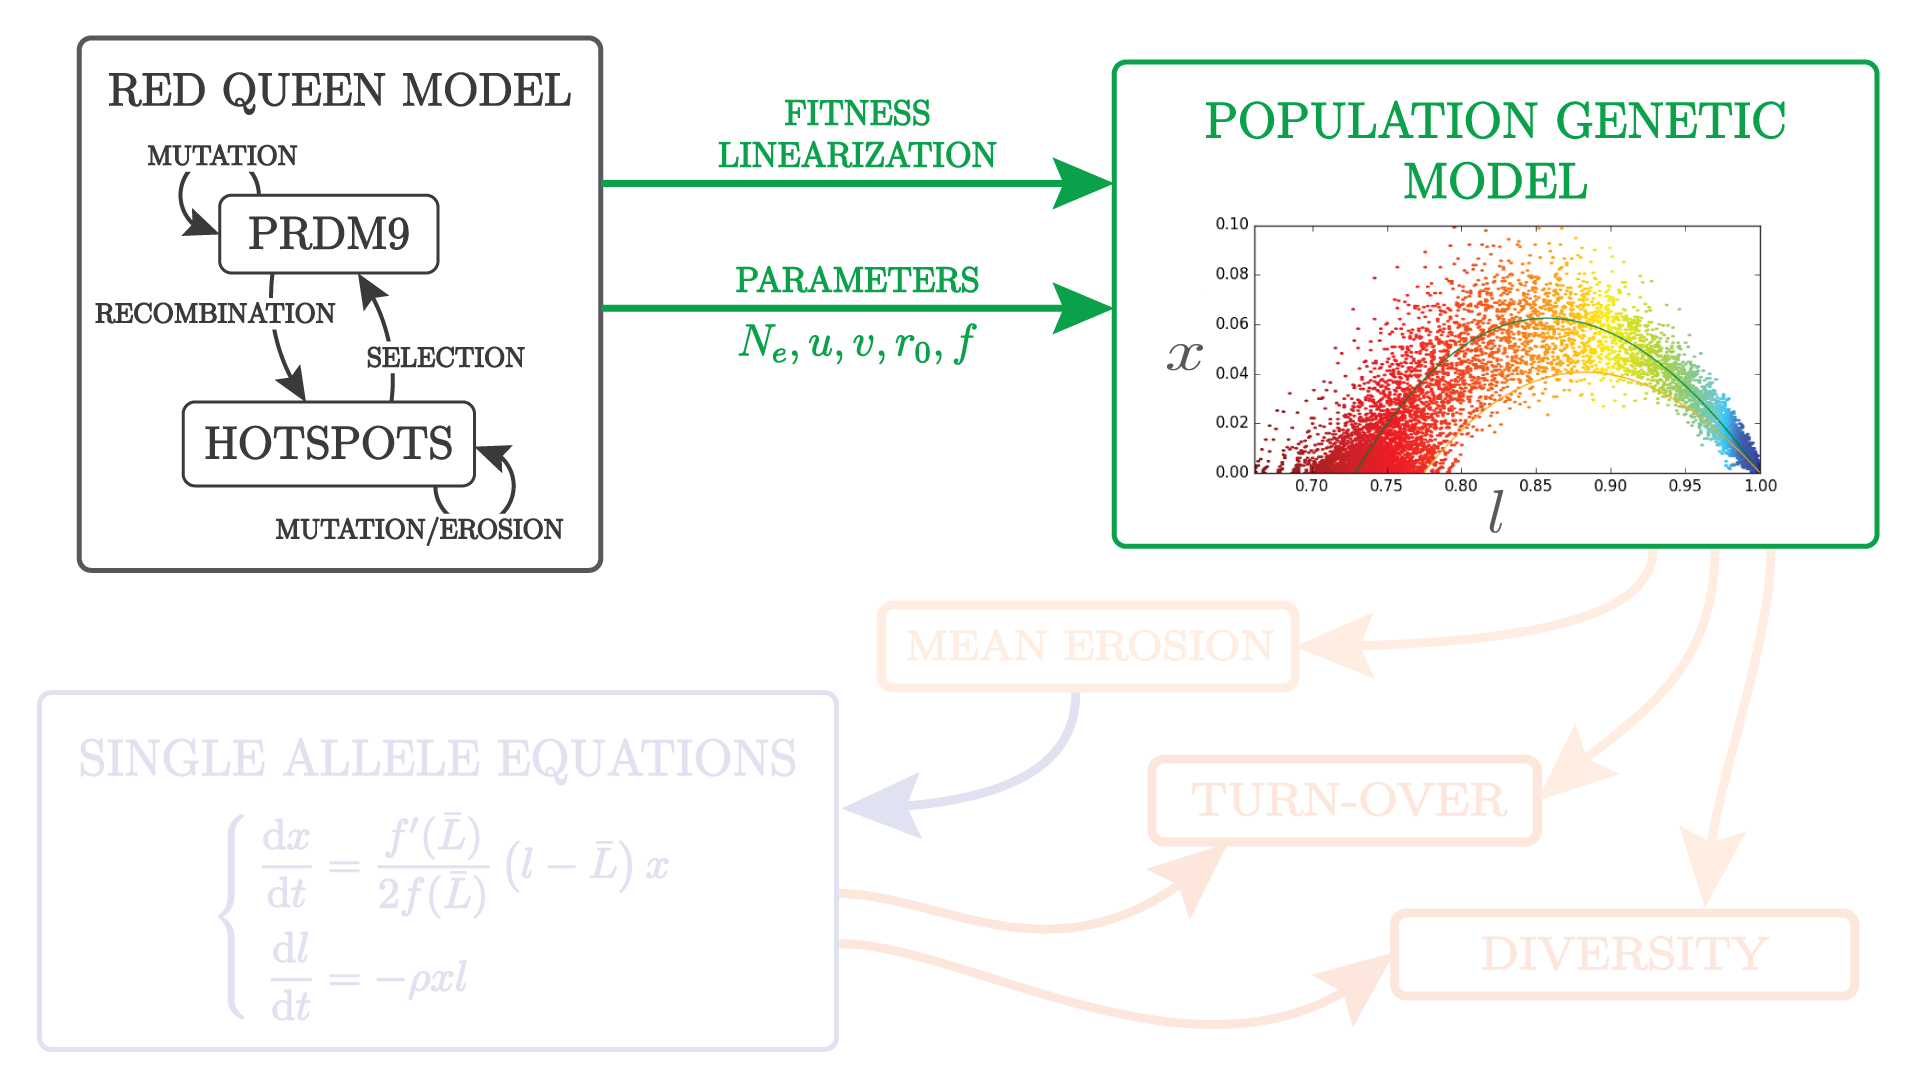
\includegraphics[width=8.5cm]{Images/overline-2.png}
	\end{center}
\end{frame}

\begin{frame}
	\frametitle{Parameters}
	\begin{center}
       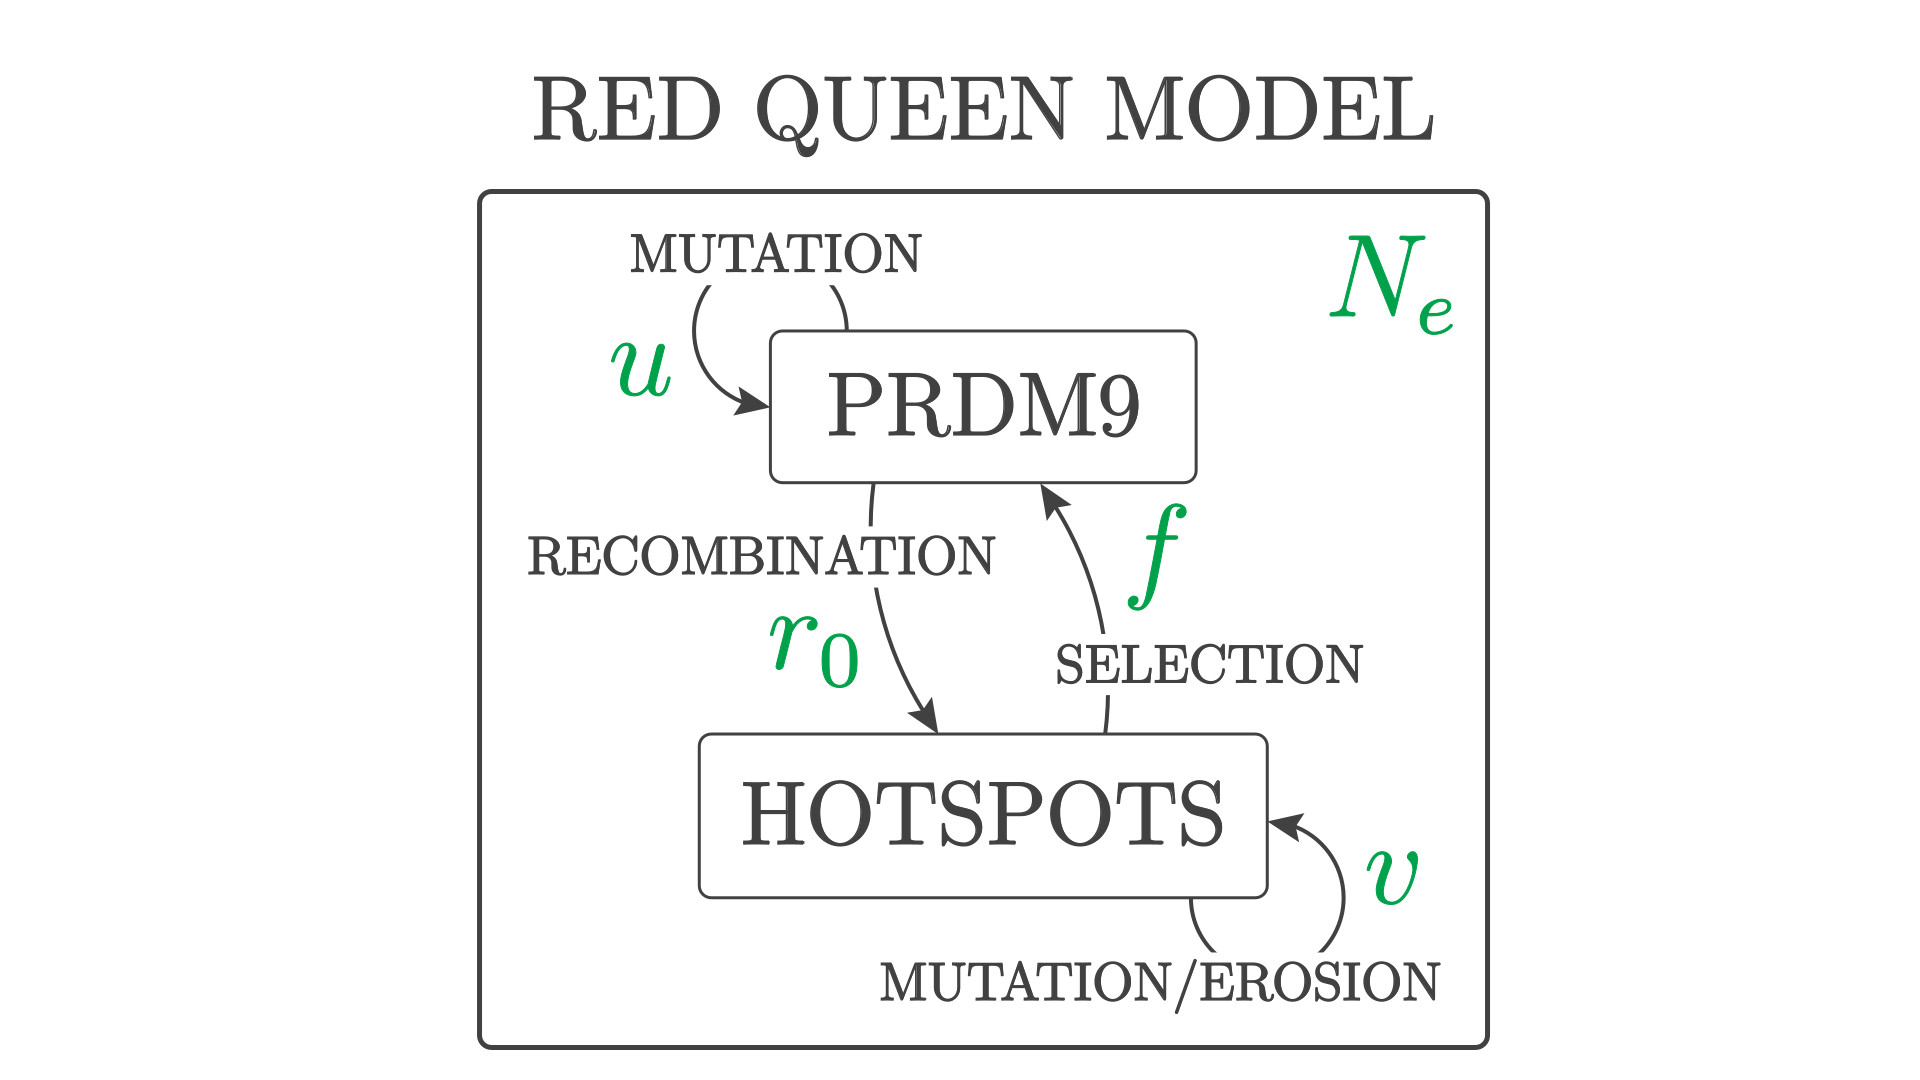
\includegraphics[width=9cm]{Images/red-queen-model.jpg}
	\end{center}
\end{frame}

\begin{frame}
	\begin{center}
		\Large
    Erosion of the hotspots (explanation, equation)
	\end{center}
\end{frame}

\begin{frame}
	\begin{center}
		\Large
    Mutation of PRDM9, selection (explanation, equation)
	\end{center}
\end{frame}

\begin{frame}
	\begin{center}
		\Large
    Trajectory of frequency and erosion (images of simulations)
	\end{center}
\end{frame}

\section{Results}

\begin{frame}
	\begin{center}
	\huge
	Chapter 3. \\
       Results
	\end{center}
\end{frame}


\begin{frame}
\frametitle{Results}
	\begin{center}
       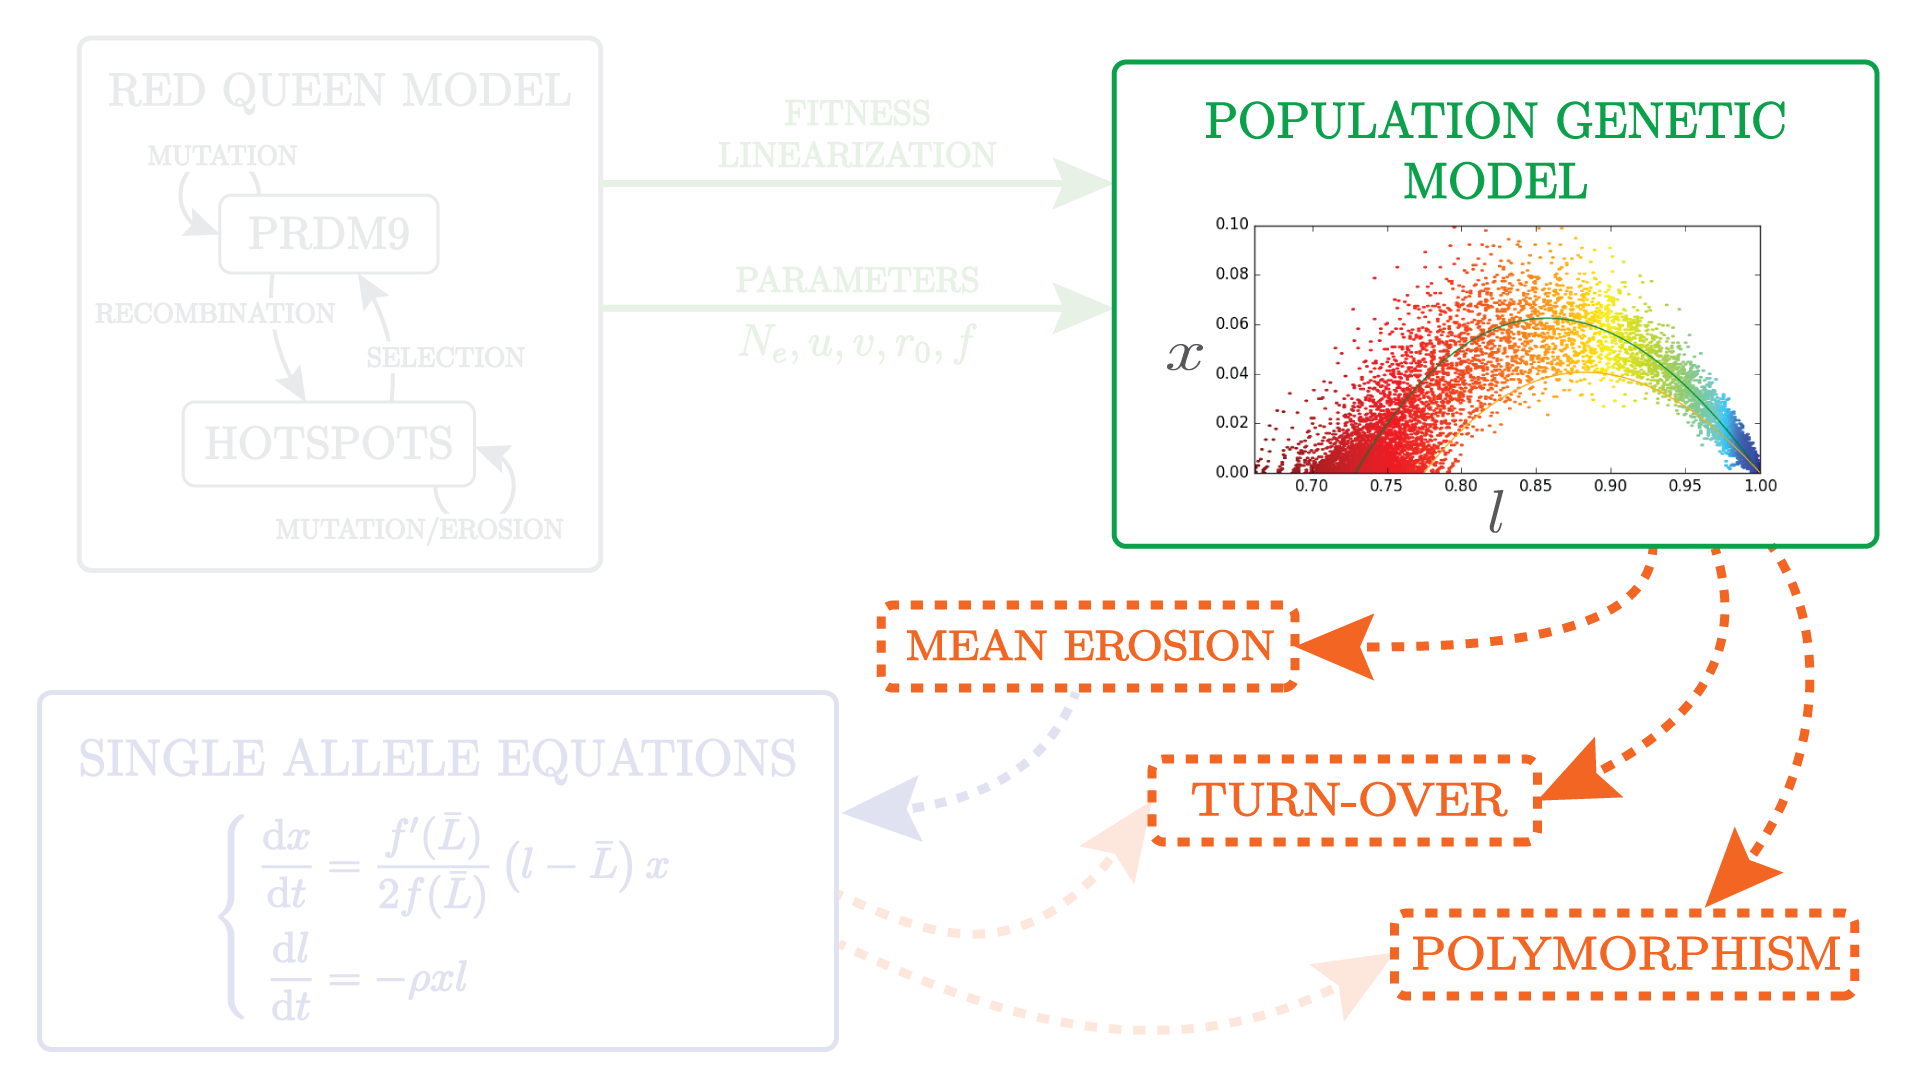
\includegraphics[width=8.5cm]{Images/overline-3.png}
	\end{center}
\end{frame}

\begin{frame}
	\begin{center}
	\Large
    Define $K_e$ and see evolution of $K_e$ with $N_e$
	\end{center}
\end{frame}

\begin{frame}
	\begin{center}
		\Large
    	Polymorphism of PRDM9
	\end{center}
	$ u $ is the mutation rate of PRDM9. \\
	$ N_e $ is the population size. \\ 
	\begin{enumerate}
		\item $u N_e \ll 1 \Rightarrow  $ single allele succession.
		\item $u N_e \gg 1 \Rightarrow  $ polymorphism.
		
		\item $\nearrow$ with regard to $u$ and $N_e$.
		
		\item $\rightsquigarrow$ with regard to the mutation ($v$) and recombination rate at the hotspots ($r_o$)
		
		\item $\rightsquigarrow$ with regard to the fitness function.
	\end{enumerate}
\end{frame}

\begin{frame}
	\begin{center}
       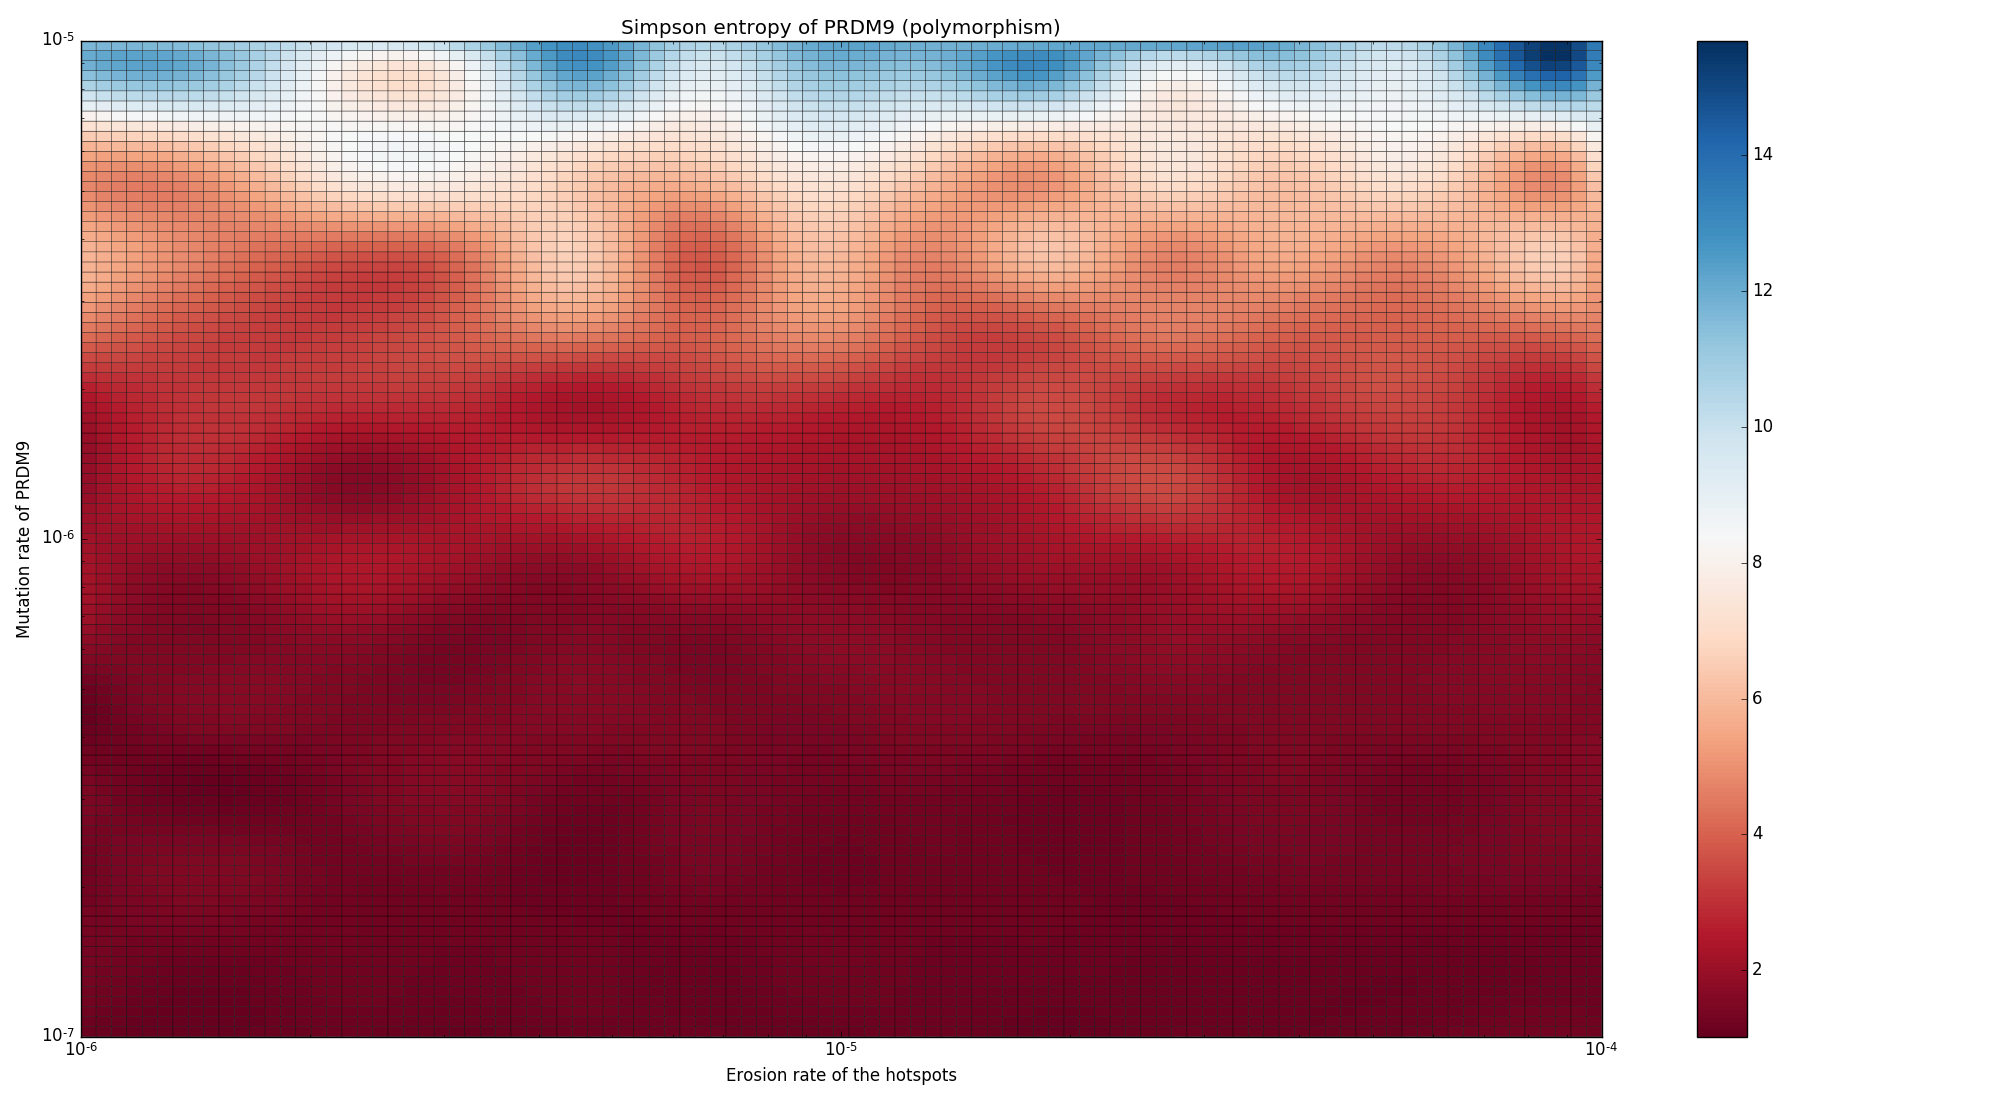
\includegraphics[width=11cm]{Images/simpson-entropy-mutation-erosion.png}
	\end{center}
\end{frame}


\begin{frame}
	\begin{center}
       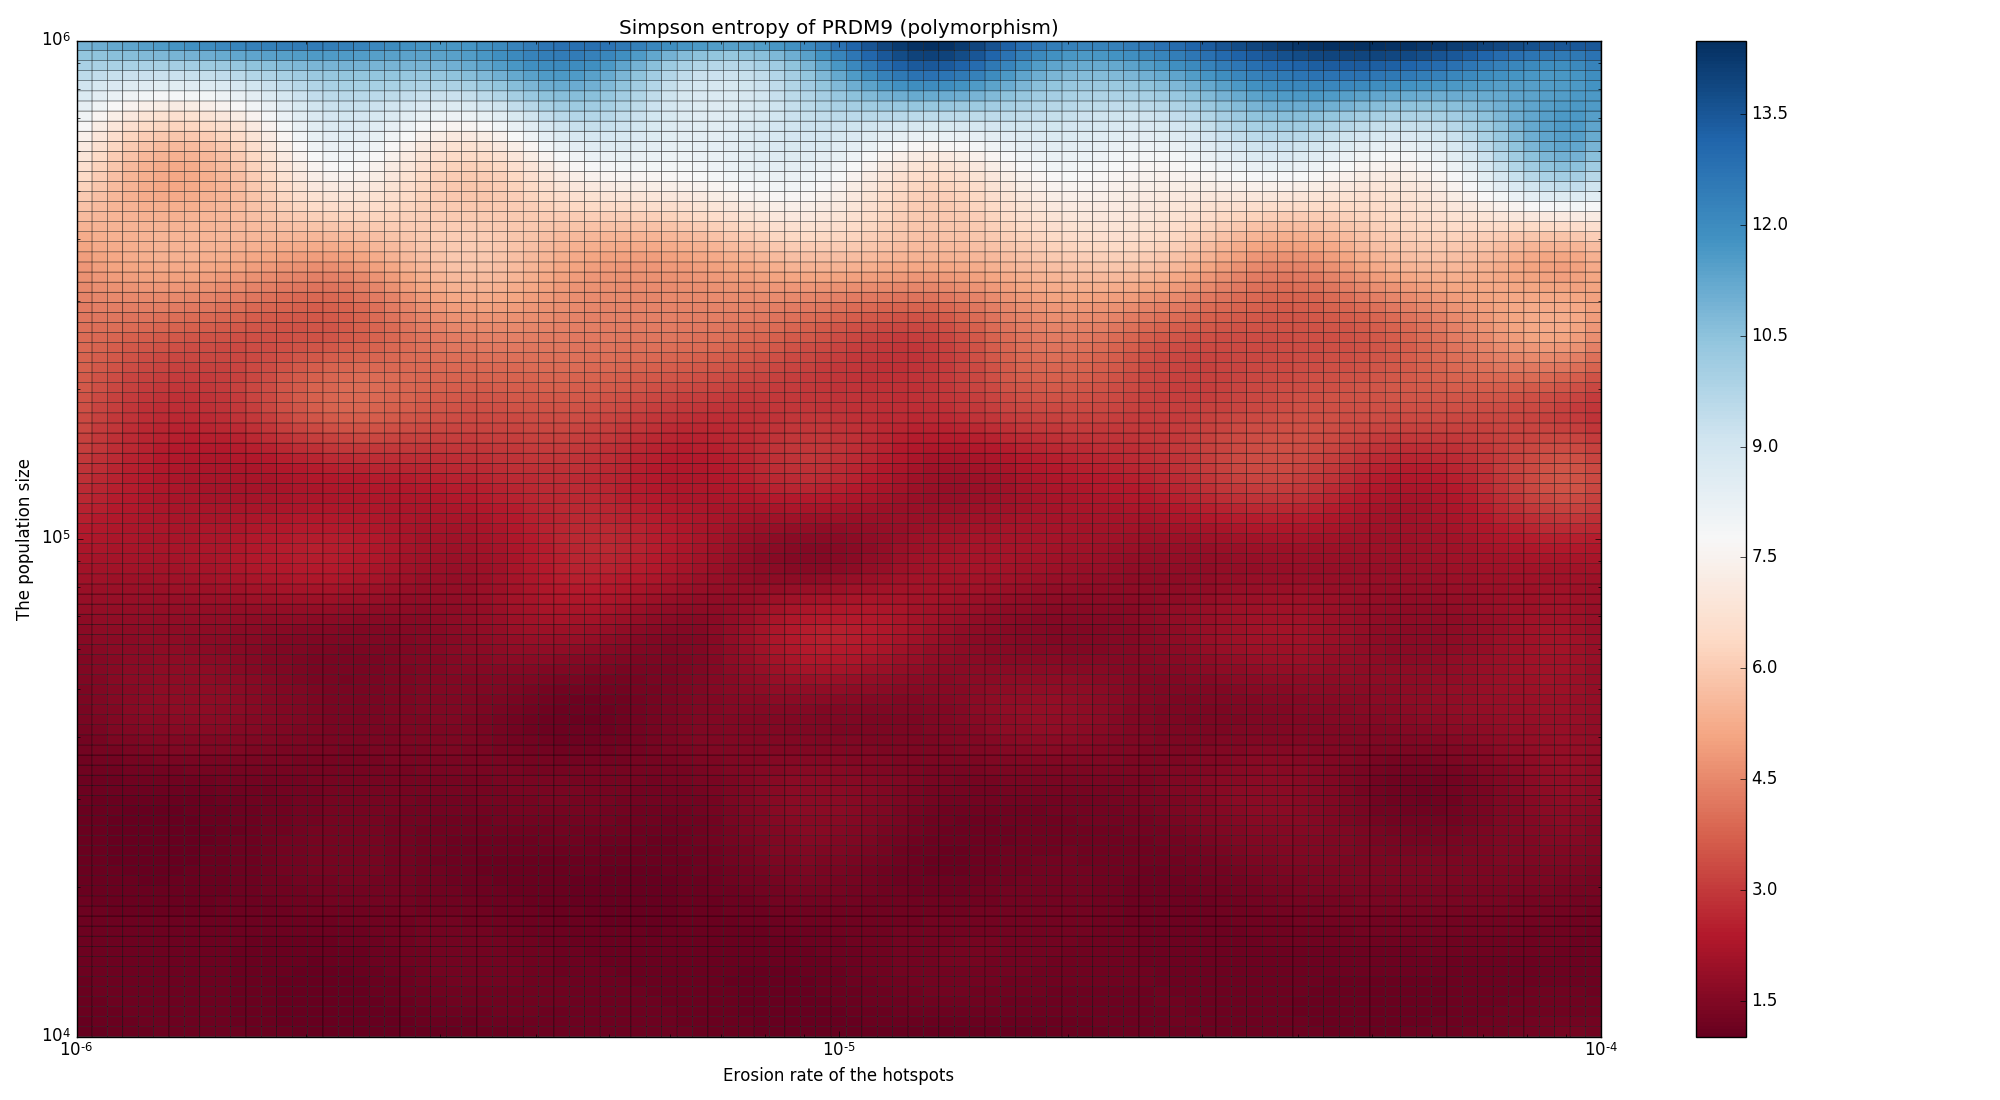
\includegraphics[width=11cm]{Images/simpson-entropy-population-erosion.png}
	\end{center}
\end{frame}

\begin{frame}
	\begin{center}
       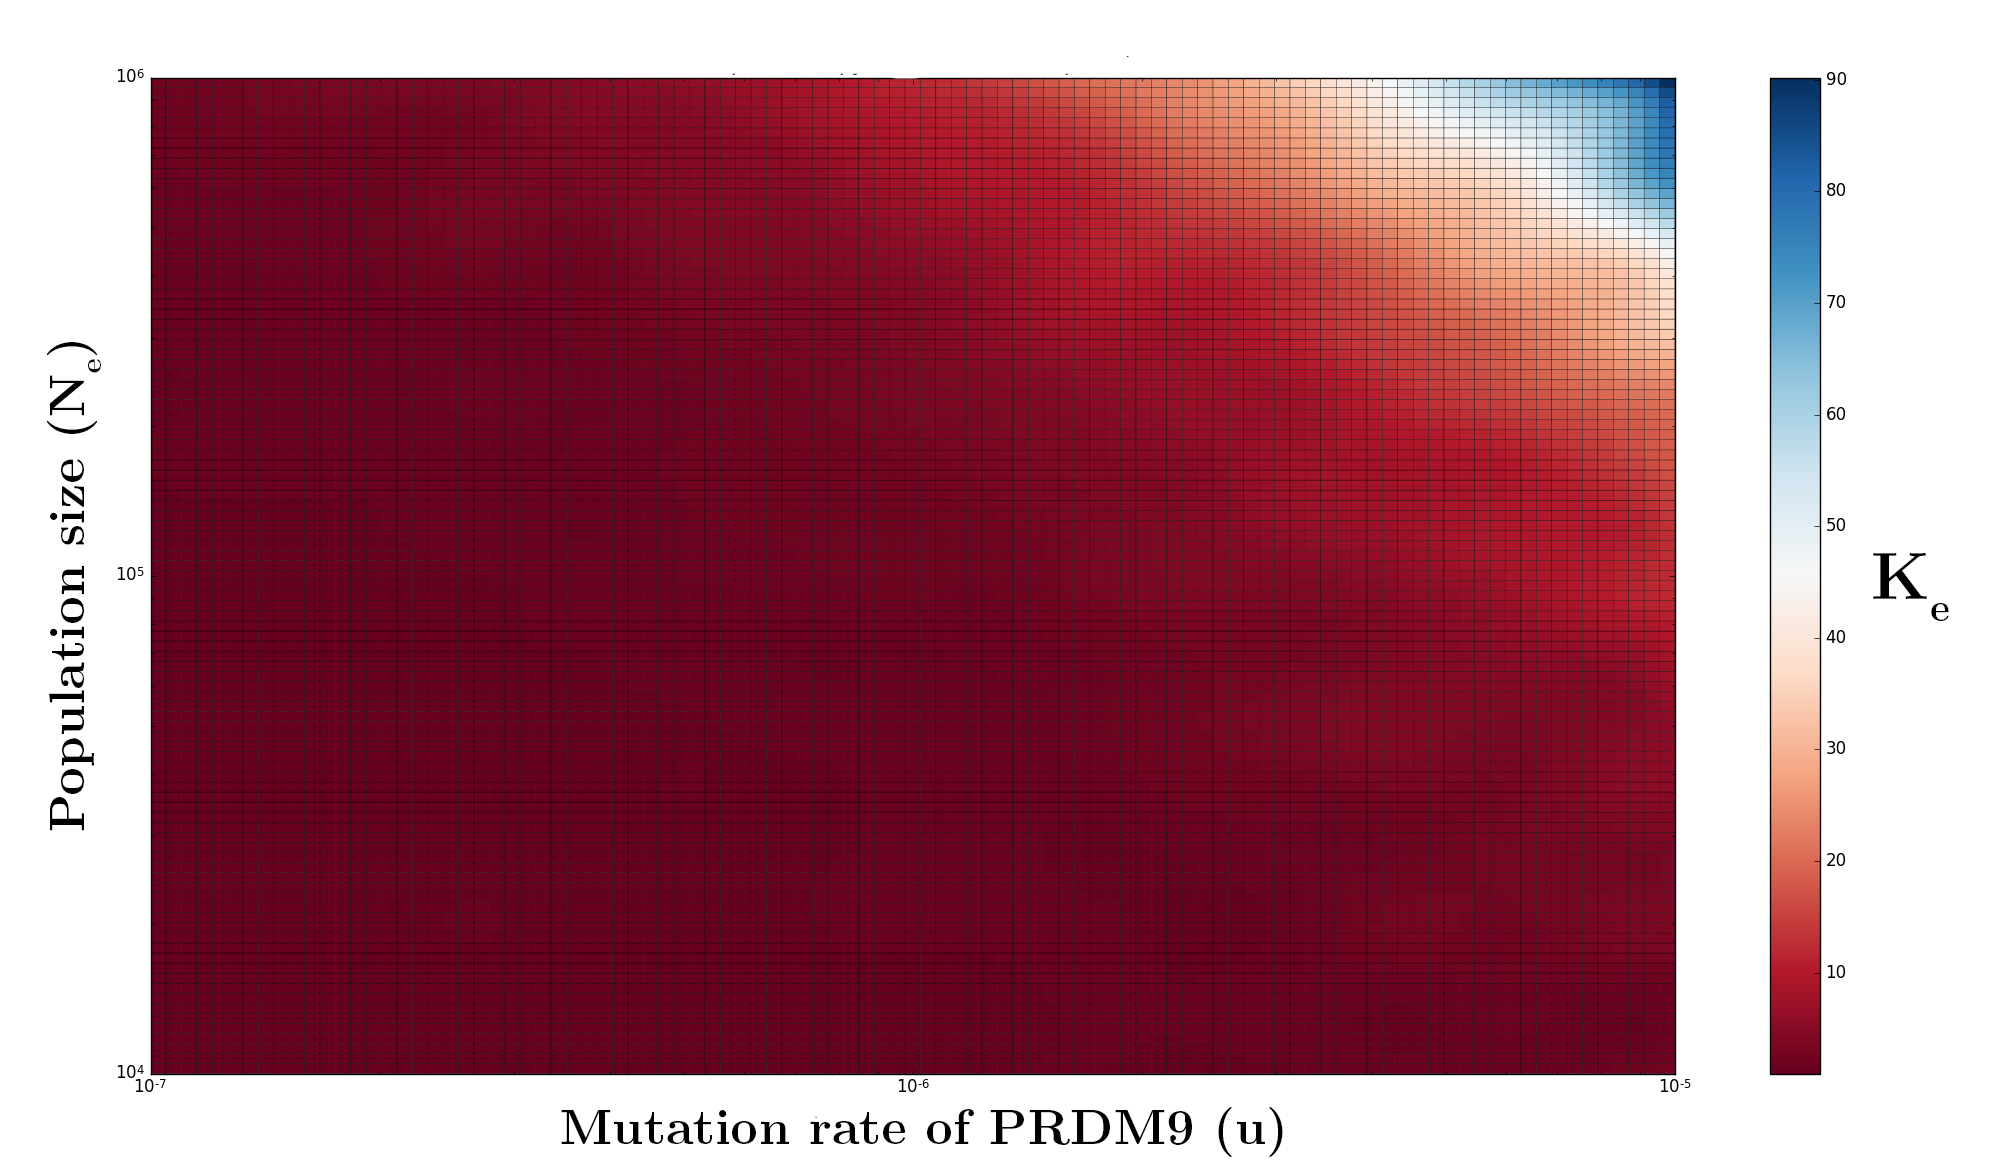
\includegraphics[width=11cm]{Images/simpson-entropy-population-mutation.png}
	\end{center}
\end{frame}


\begin{frame}
	\begin{center}
	\Large
    Define $\bar{L}$ and see evolution of $\bar{L}$ with $N_e$
	\end{center}
\end{frame}

\begin{frame}
	\begin{center}
		\Large
    	Mean erosion of the hotspots
	\end{center}
	\begin{enumerate}
		\item $\nearrow$ with regard to the mutation ($v$) and recombination rate at the hotspots ($r_o$).
		
		\item $\searrow$ with regard to mutation rate of PRDM9. ($u$).
		
		\item $\rightsquigarrow$ with regard to the population size ($N_e$).
		
		\item 	The fitness function can be linearised around the mean erosion.
	\end{enumerate}
\end{frame}

\begin{frame}
	\begin{center}
       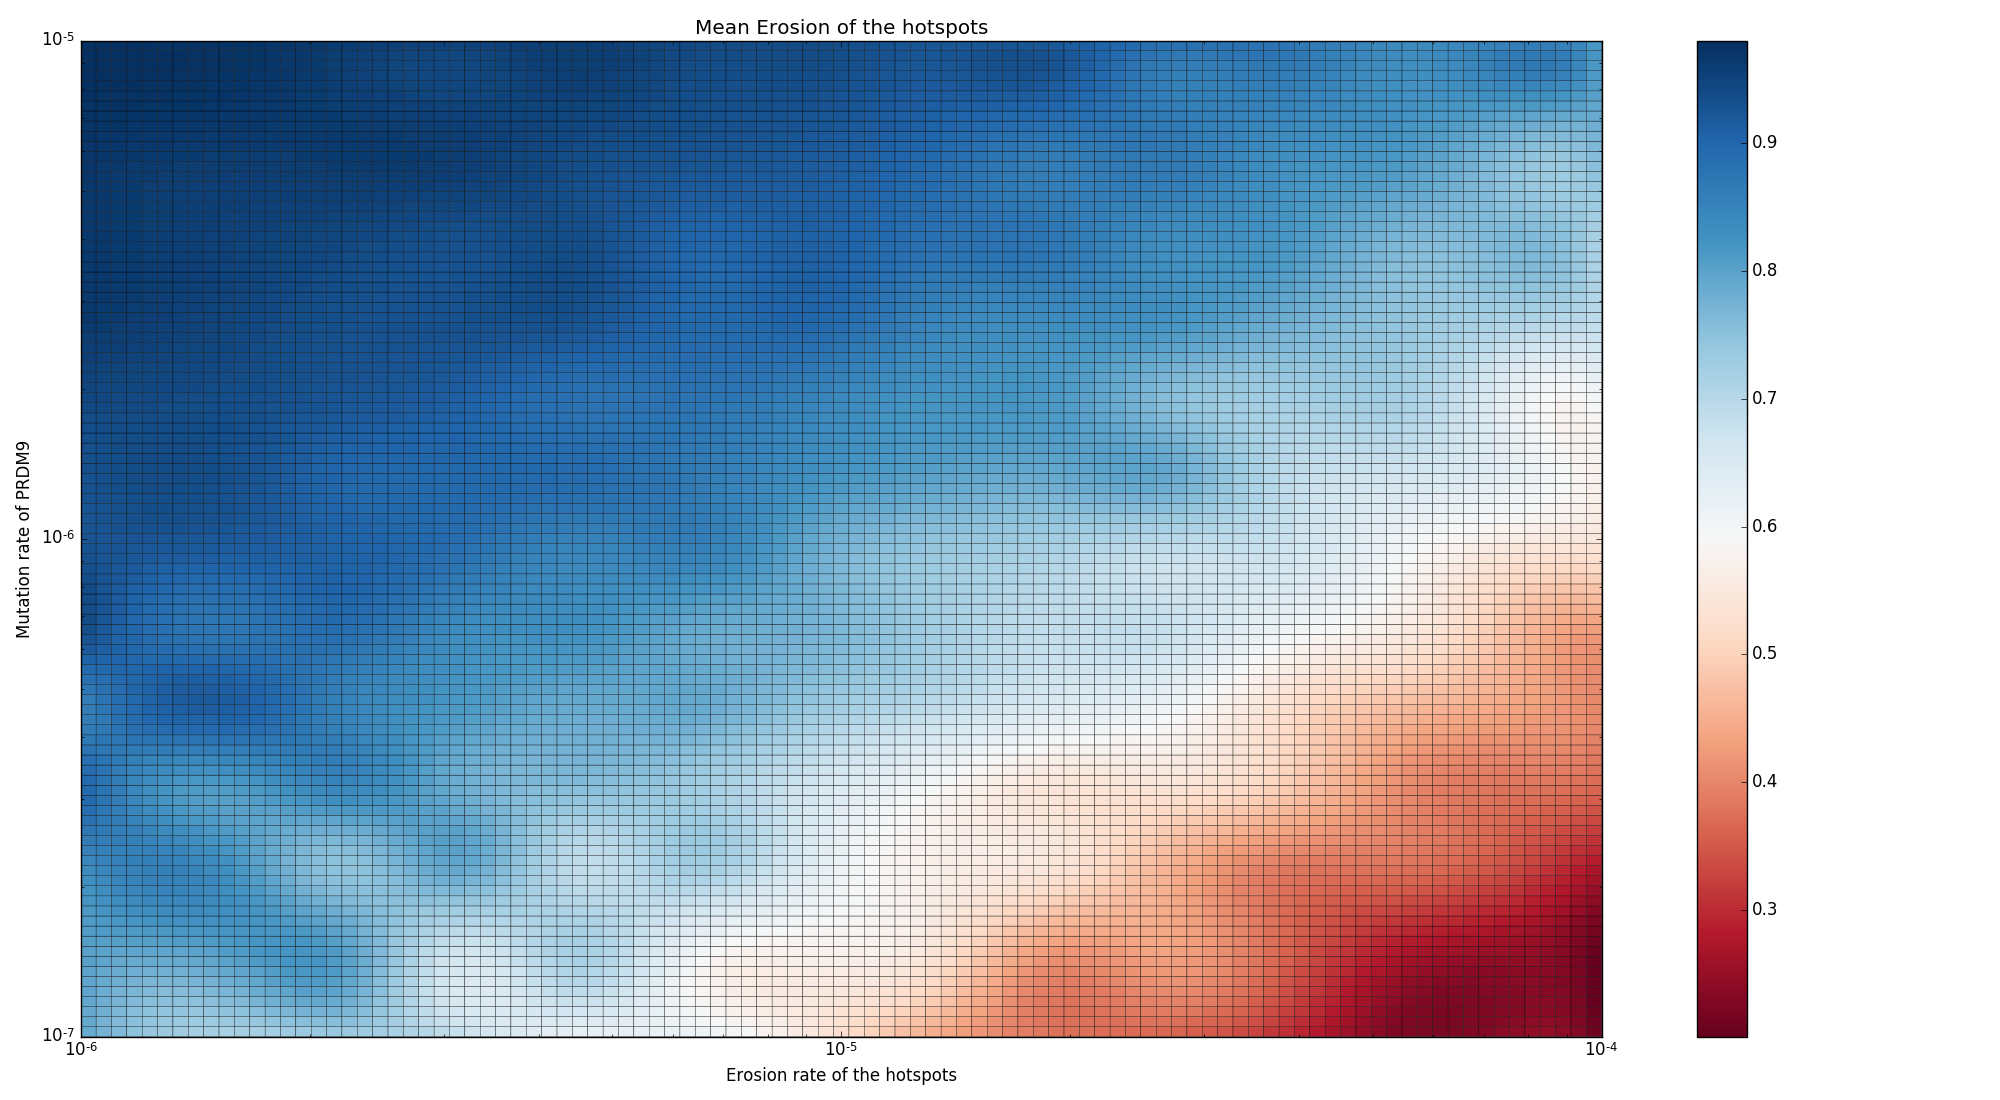
\includegraphics[width=11cm]{Images/mean-erosion-mutation-erosion.png}
	\end{center}
\end{frame}

\begin{frame}
	\begin{center}
       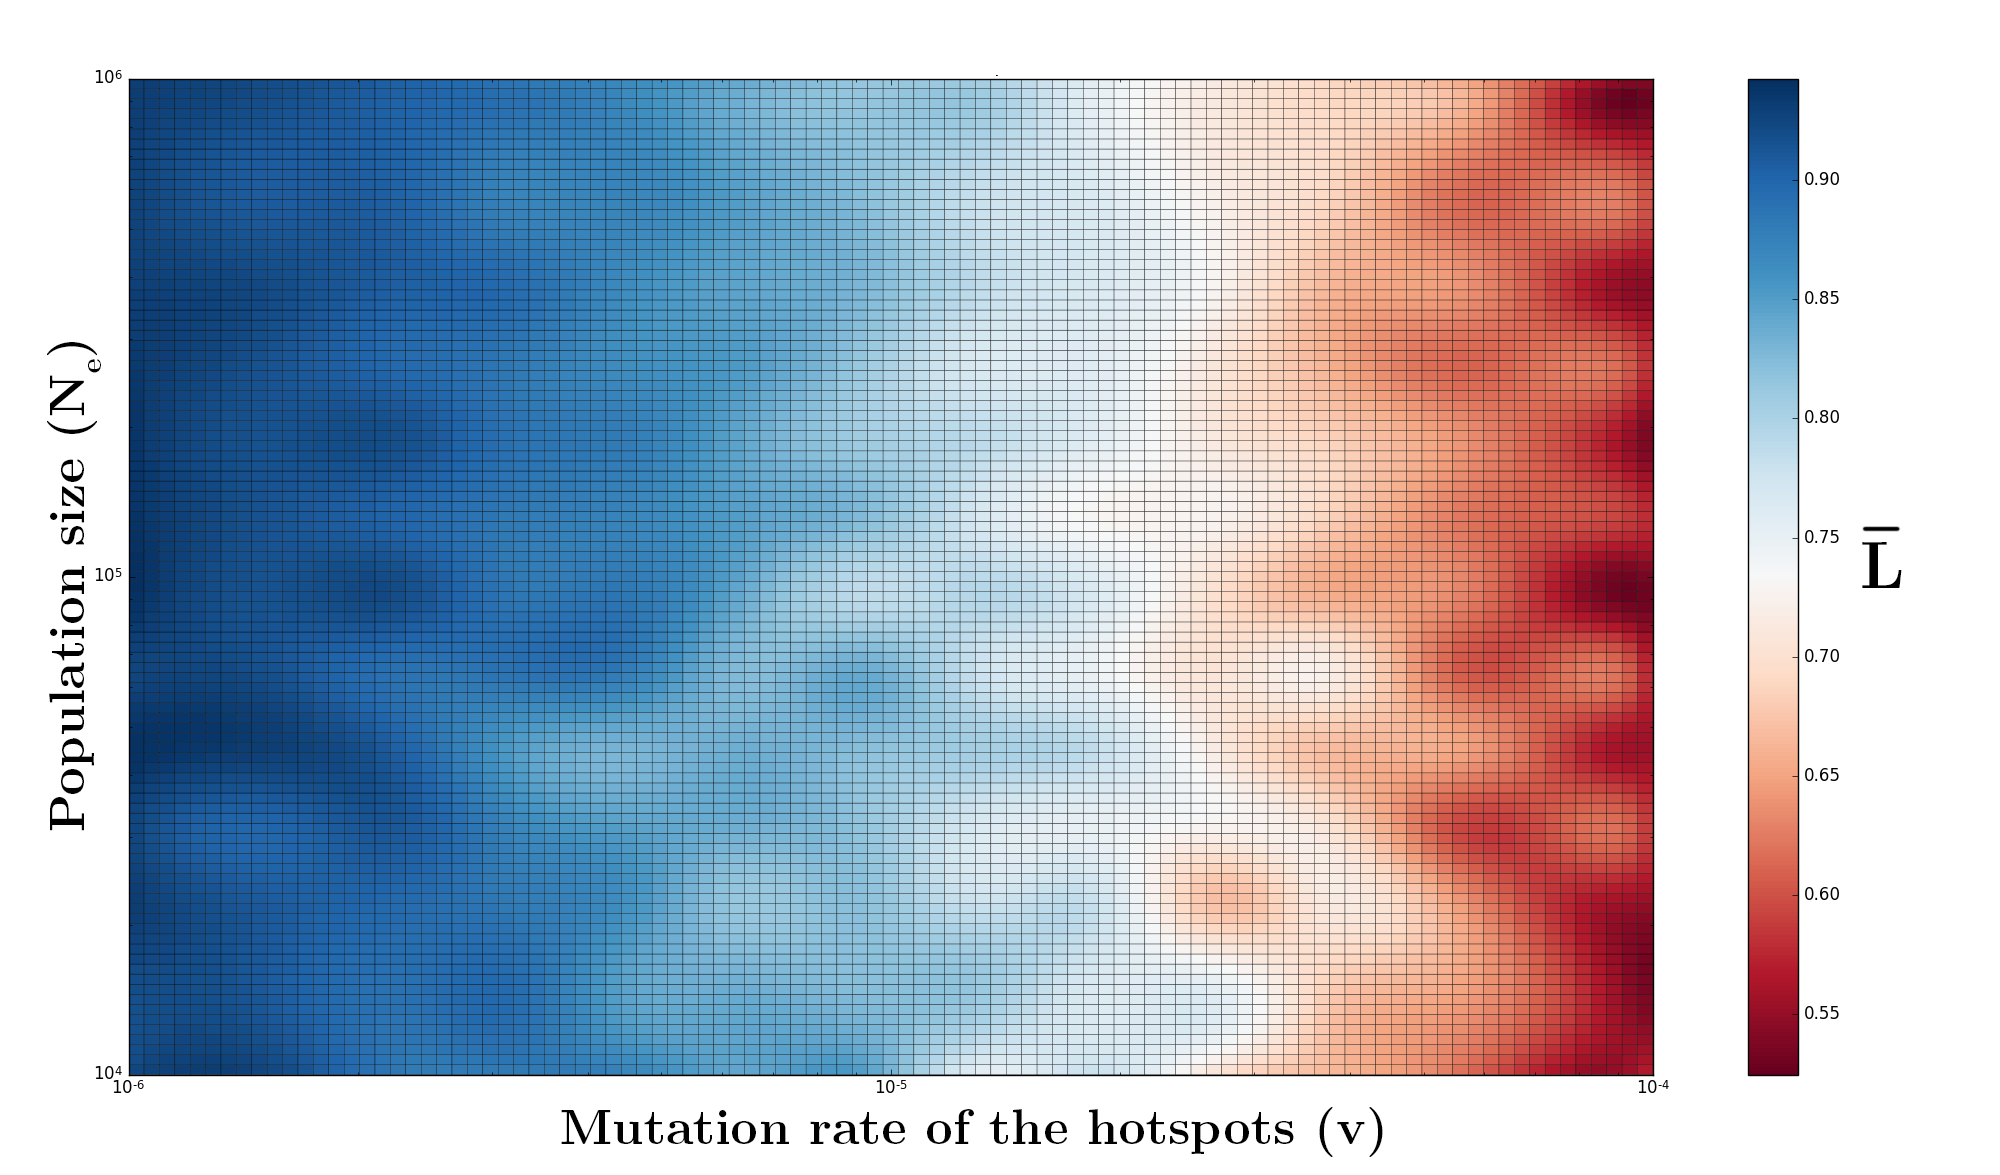
\includegraphics[width=11cm]{Images/mean-erosion-population-erosion.png}
	\end{center}
\end{frame}

\begin{frame}
	\begin{center}
       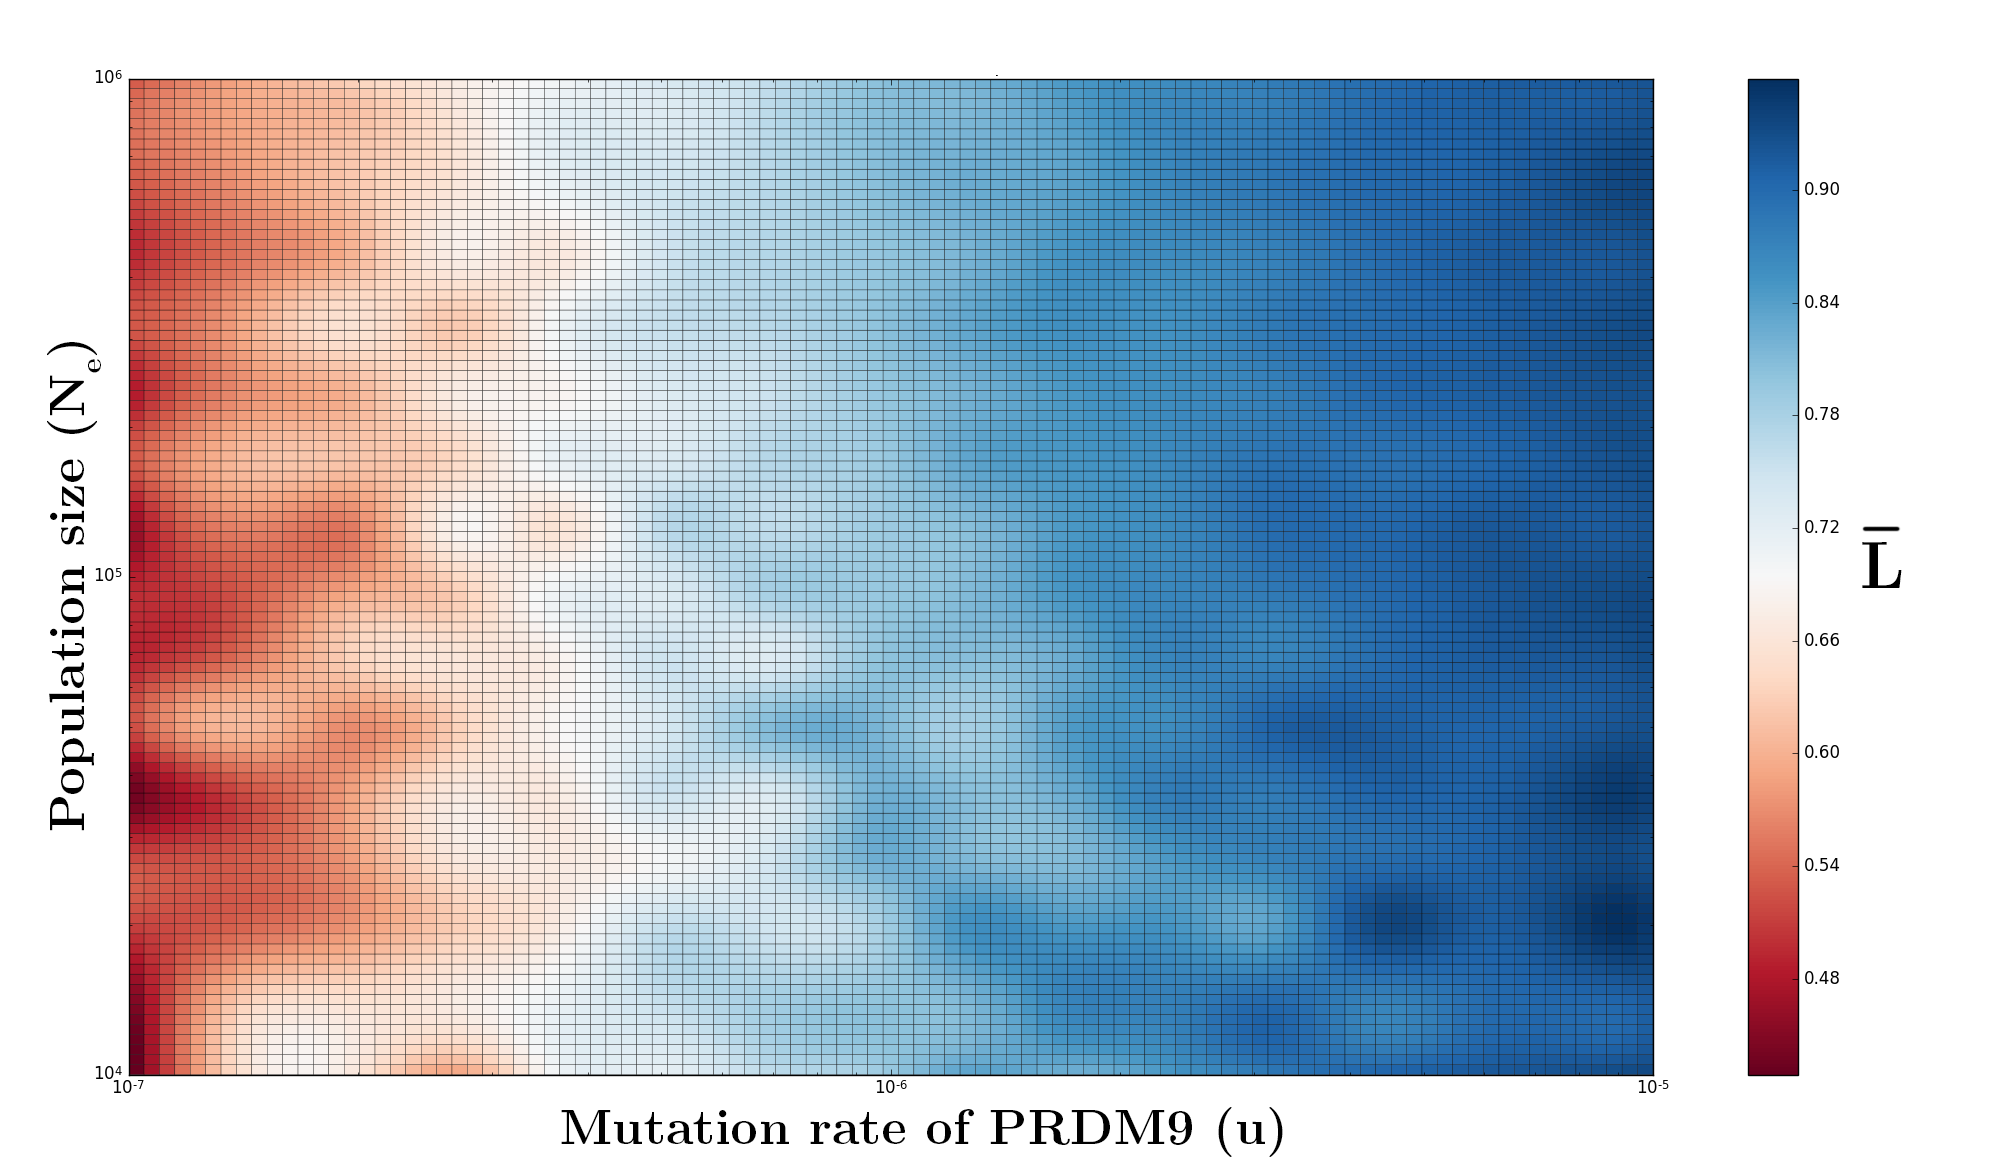
\includegraphics[width=11cm]{Images/mean-erosion-population-mutation.png}
	\end{center}
\end{frame}

\begin{frame}
	\begin{center}
	\Large
    Define $\tau$ and see evolution of $\tau$ with $N_e$
	\end{center}
\end{frame}

\begin{frame}
	\begin{center}
		\Large
    	Cross-homozygosity of the hotspots
	\end{center}
	\begin{enumerate}
		\item $\searrow$ with regard to the mutation ($v$) and recombination rate at the hotspots ($r_o$).
		
		\item $\searrow$ with regard to mutation rate of PRDM9. ($u$).
		
		\item $\searrow$ with regard to the population size ($N_e$).
		
	\end{enumerate}
\end{frame}

\begin{frame}
	\begin{center}
       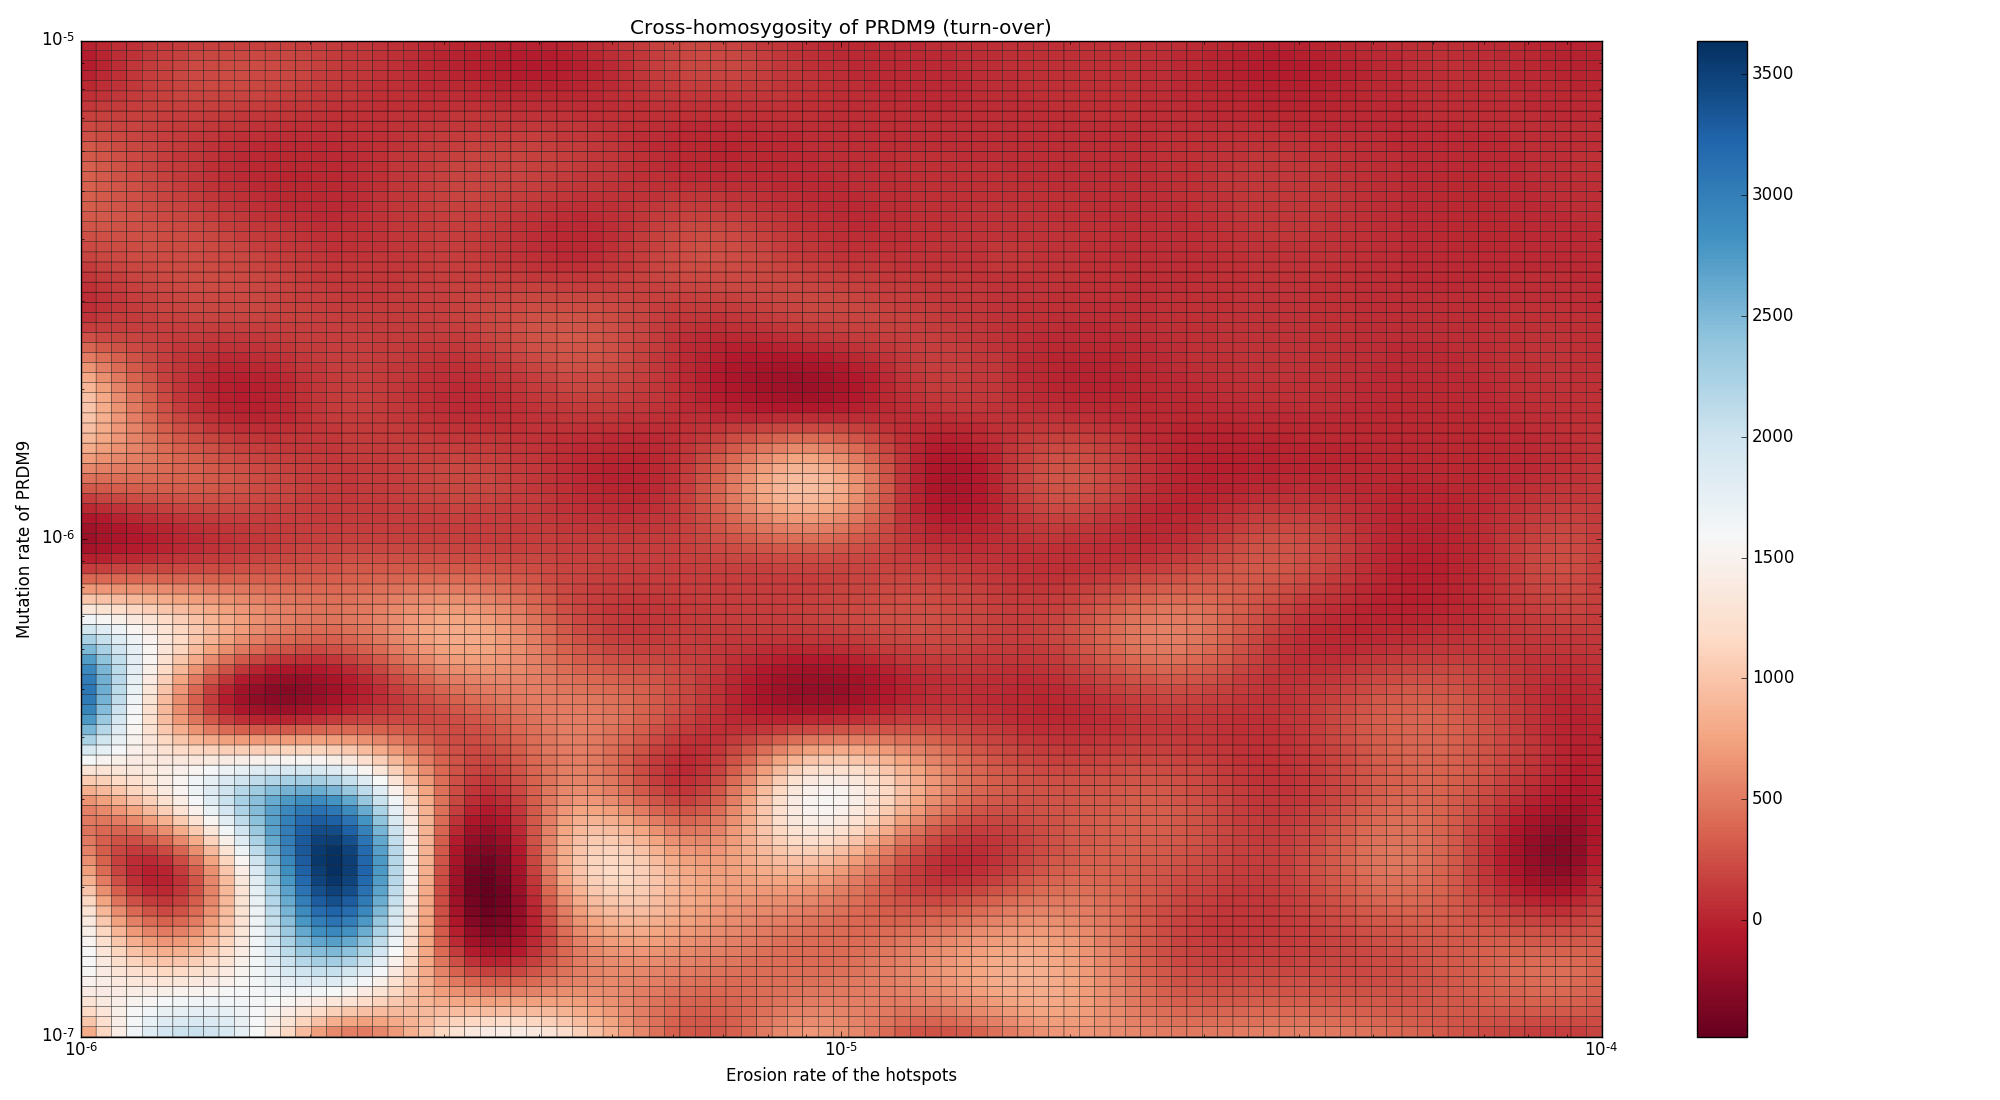
\includegraphics[width=11cm]{Images/cross-homozygosity-mutation-erosion.png}
	\end{center}
\end{frame}


\begin{frame}
	\begin{center}
       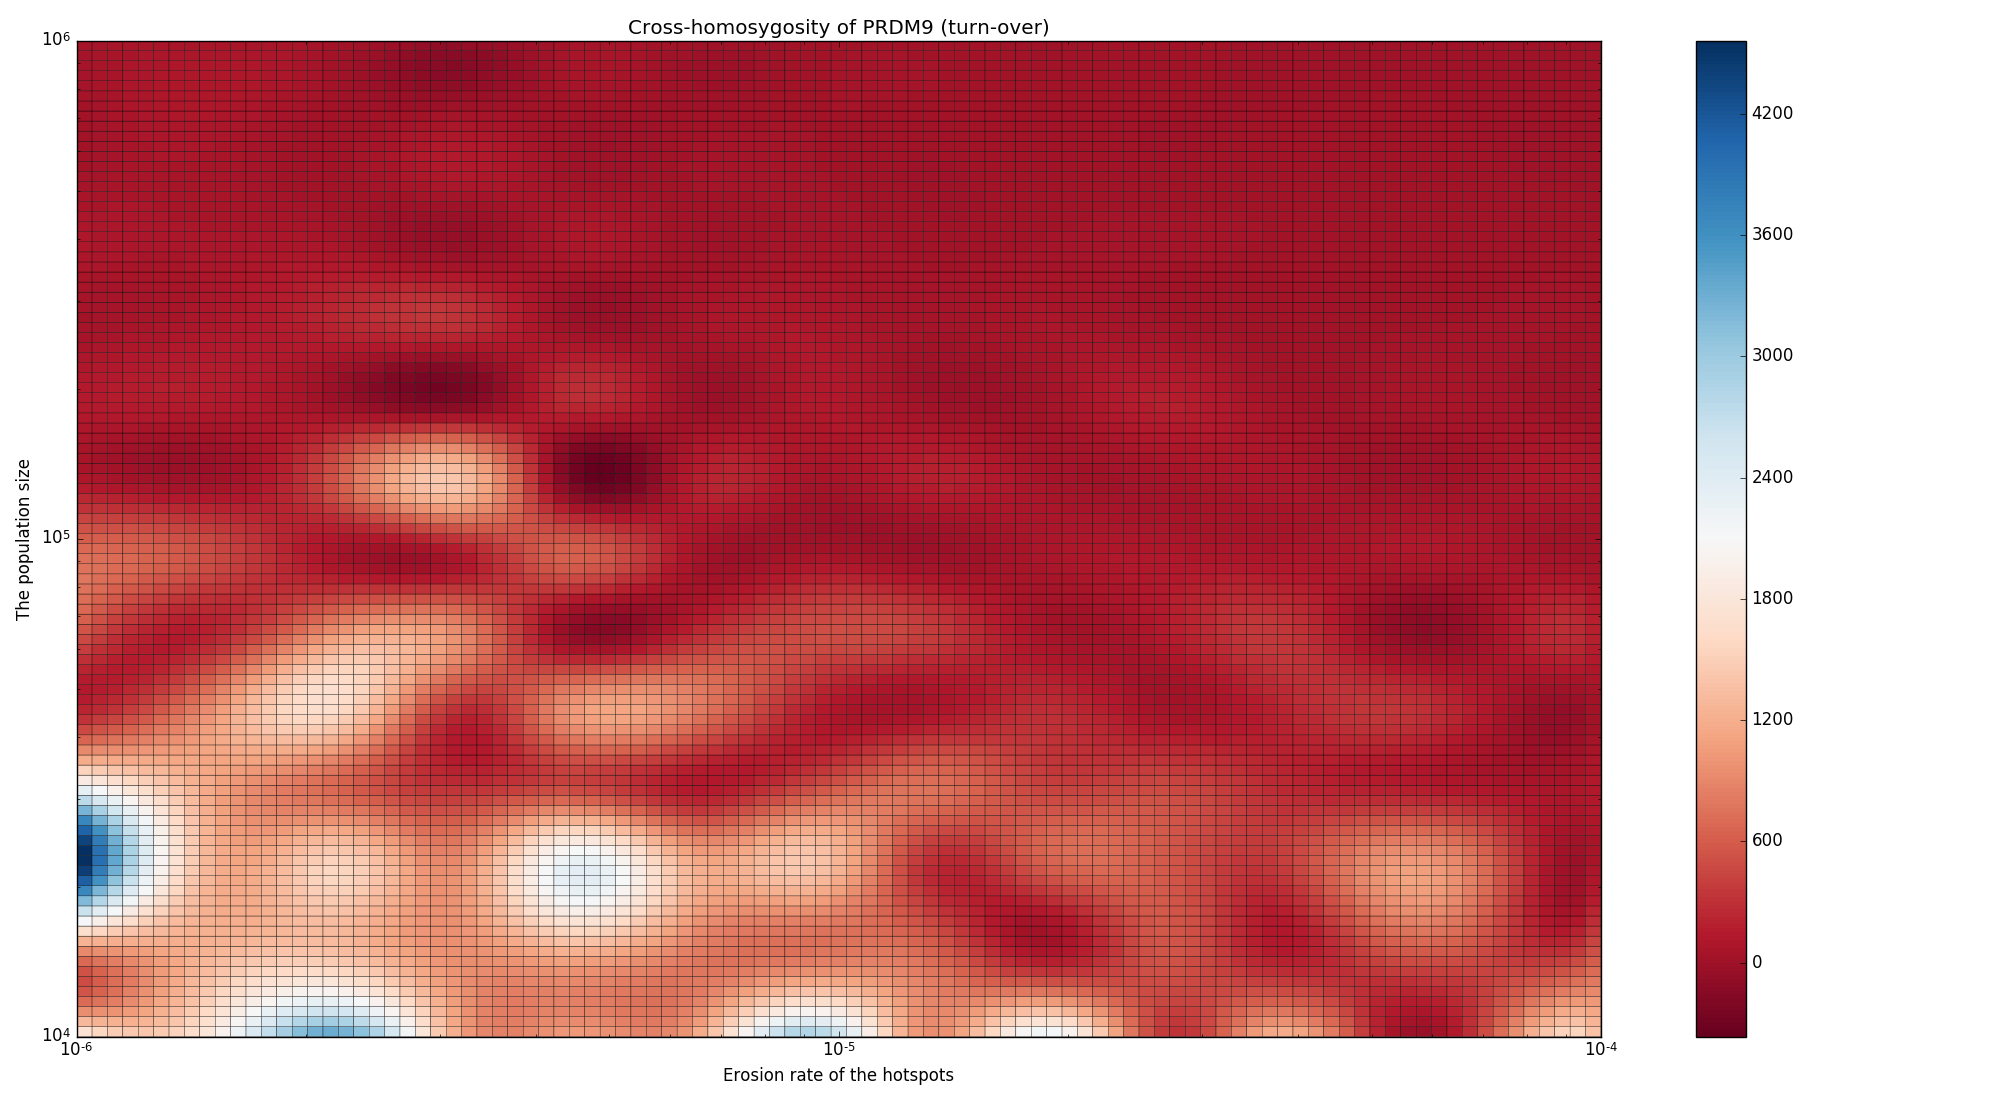
\includegraphics[width=11cm]{Images/cross-homozygosity-population-erosion.png}
	\end{center}
\end{frame}

\begin{frame}
	\begin{center}
       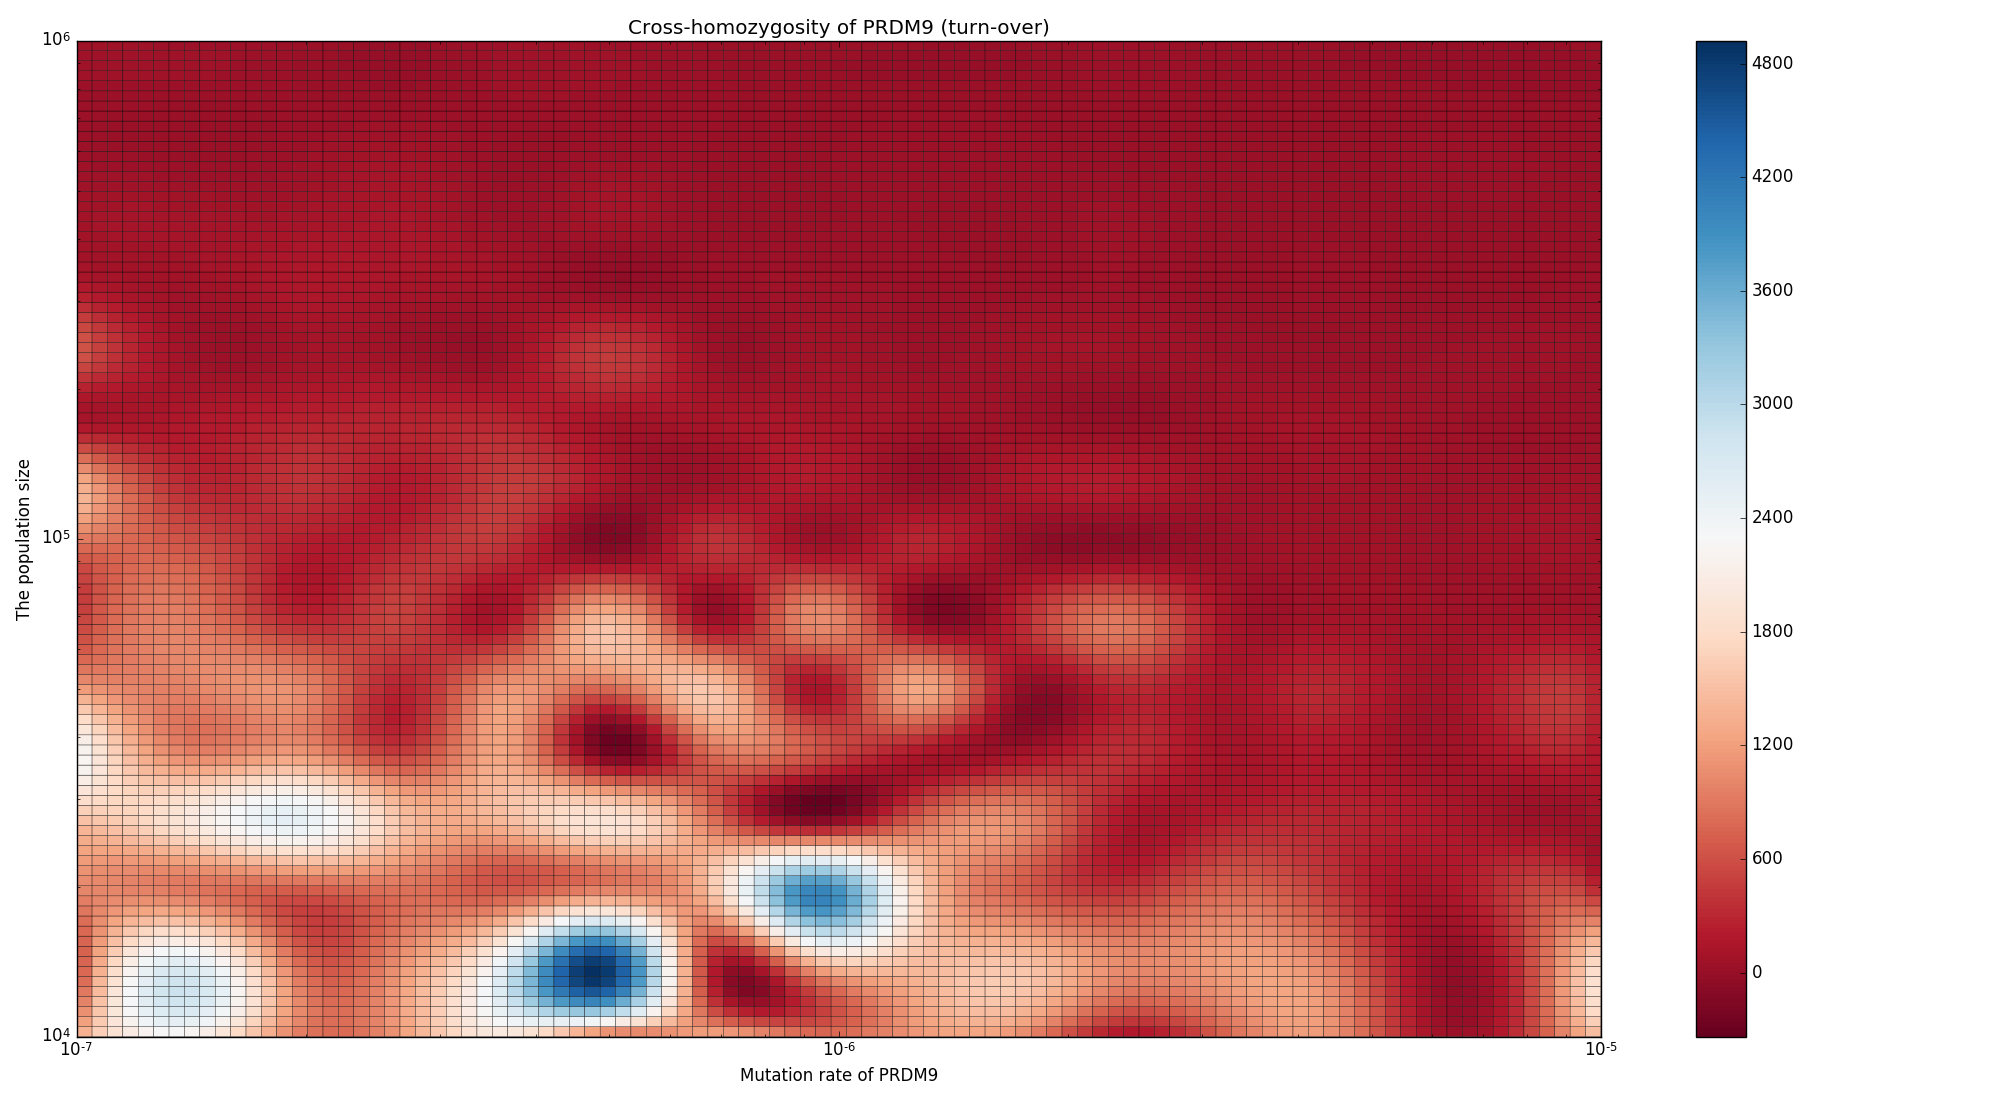
\includegraphics[width=11cm]{Images/cross-homozygosity-population-mutation.png}
	\end{center}
\end{frame}

\begin{frame}
	\begin{center}
		\Large
		Summary of results
       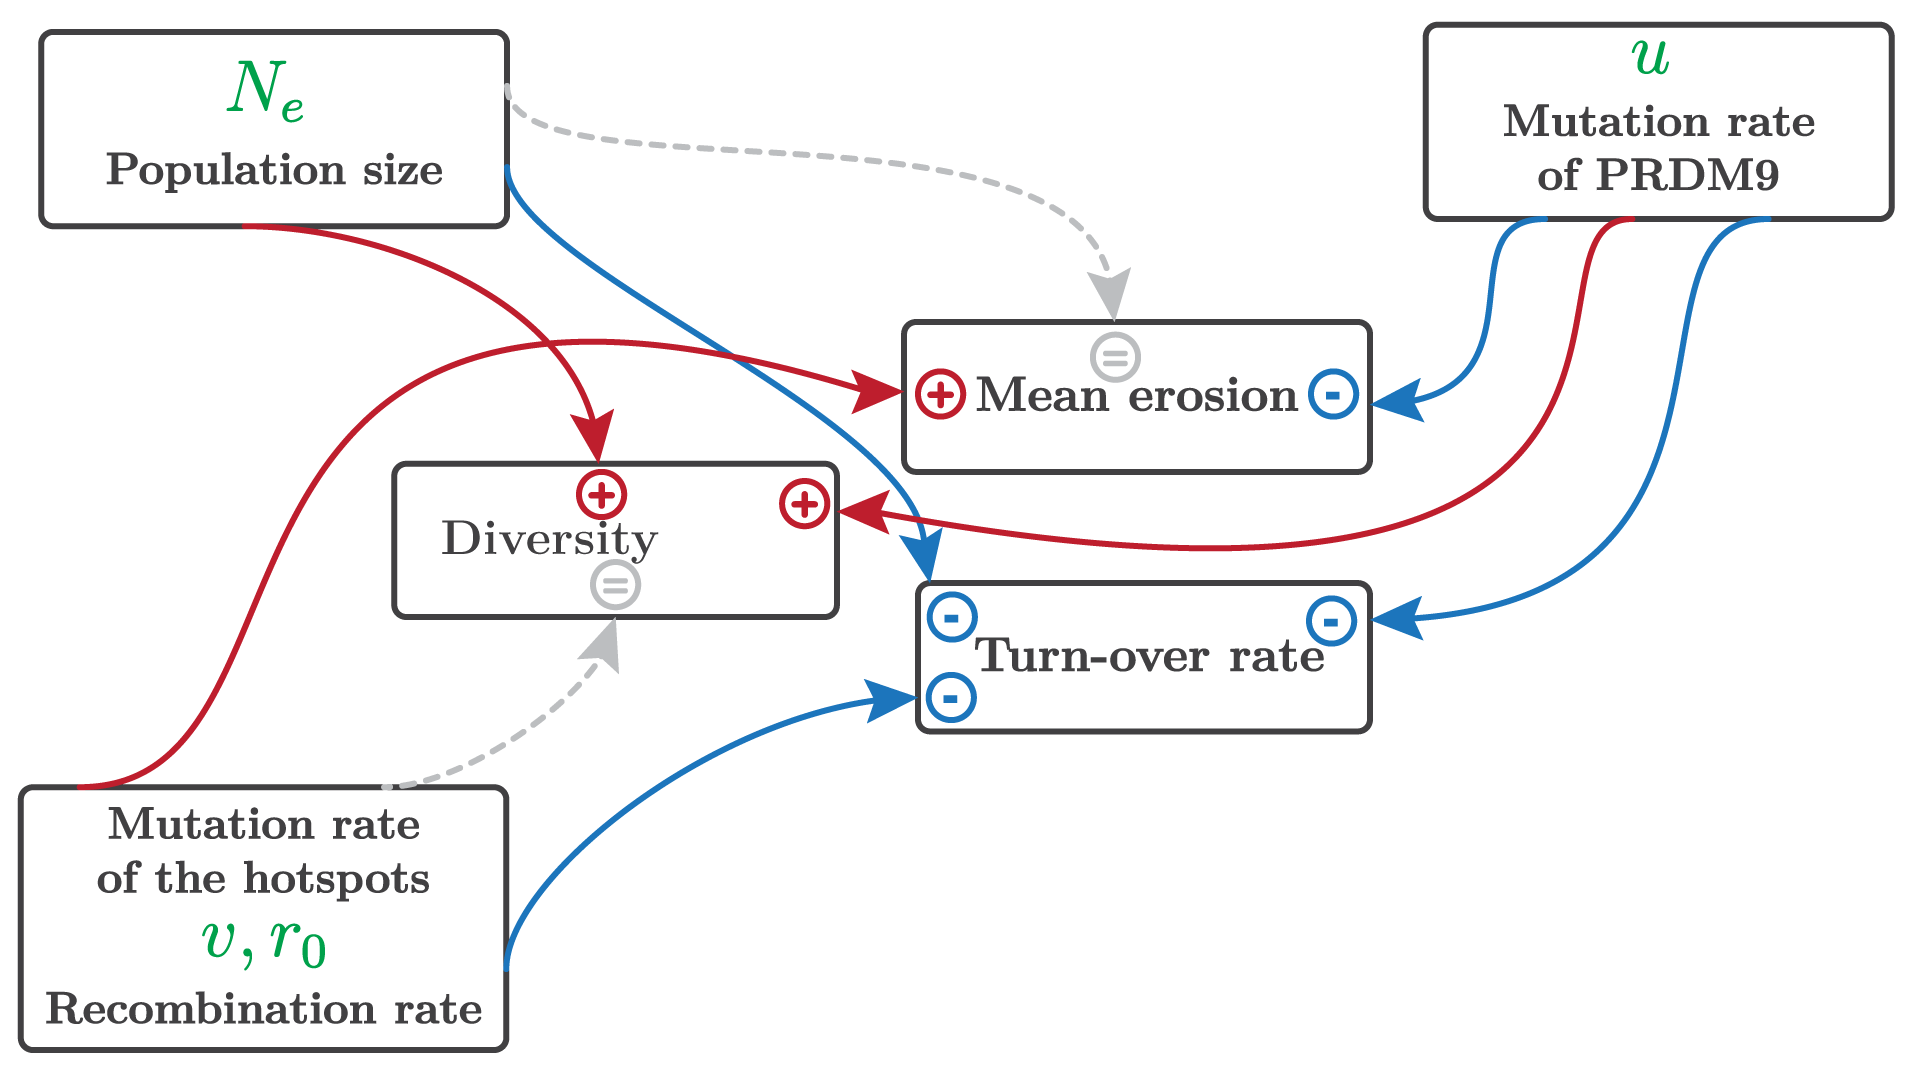
\includegraphics[width=11cm]{Images/summary.png}
	\end{center}
\end{frame}

\section{Single allele equations}

\begin{frame}
	\begin{center}
	\huge
	Chapter 4. \\
       Single allele equations
	\end{center}
\end{frame}

\begin{frame}
\frametitle{Single allele equations}
	\begin{center}
       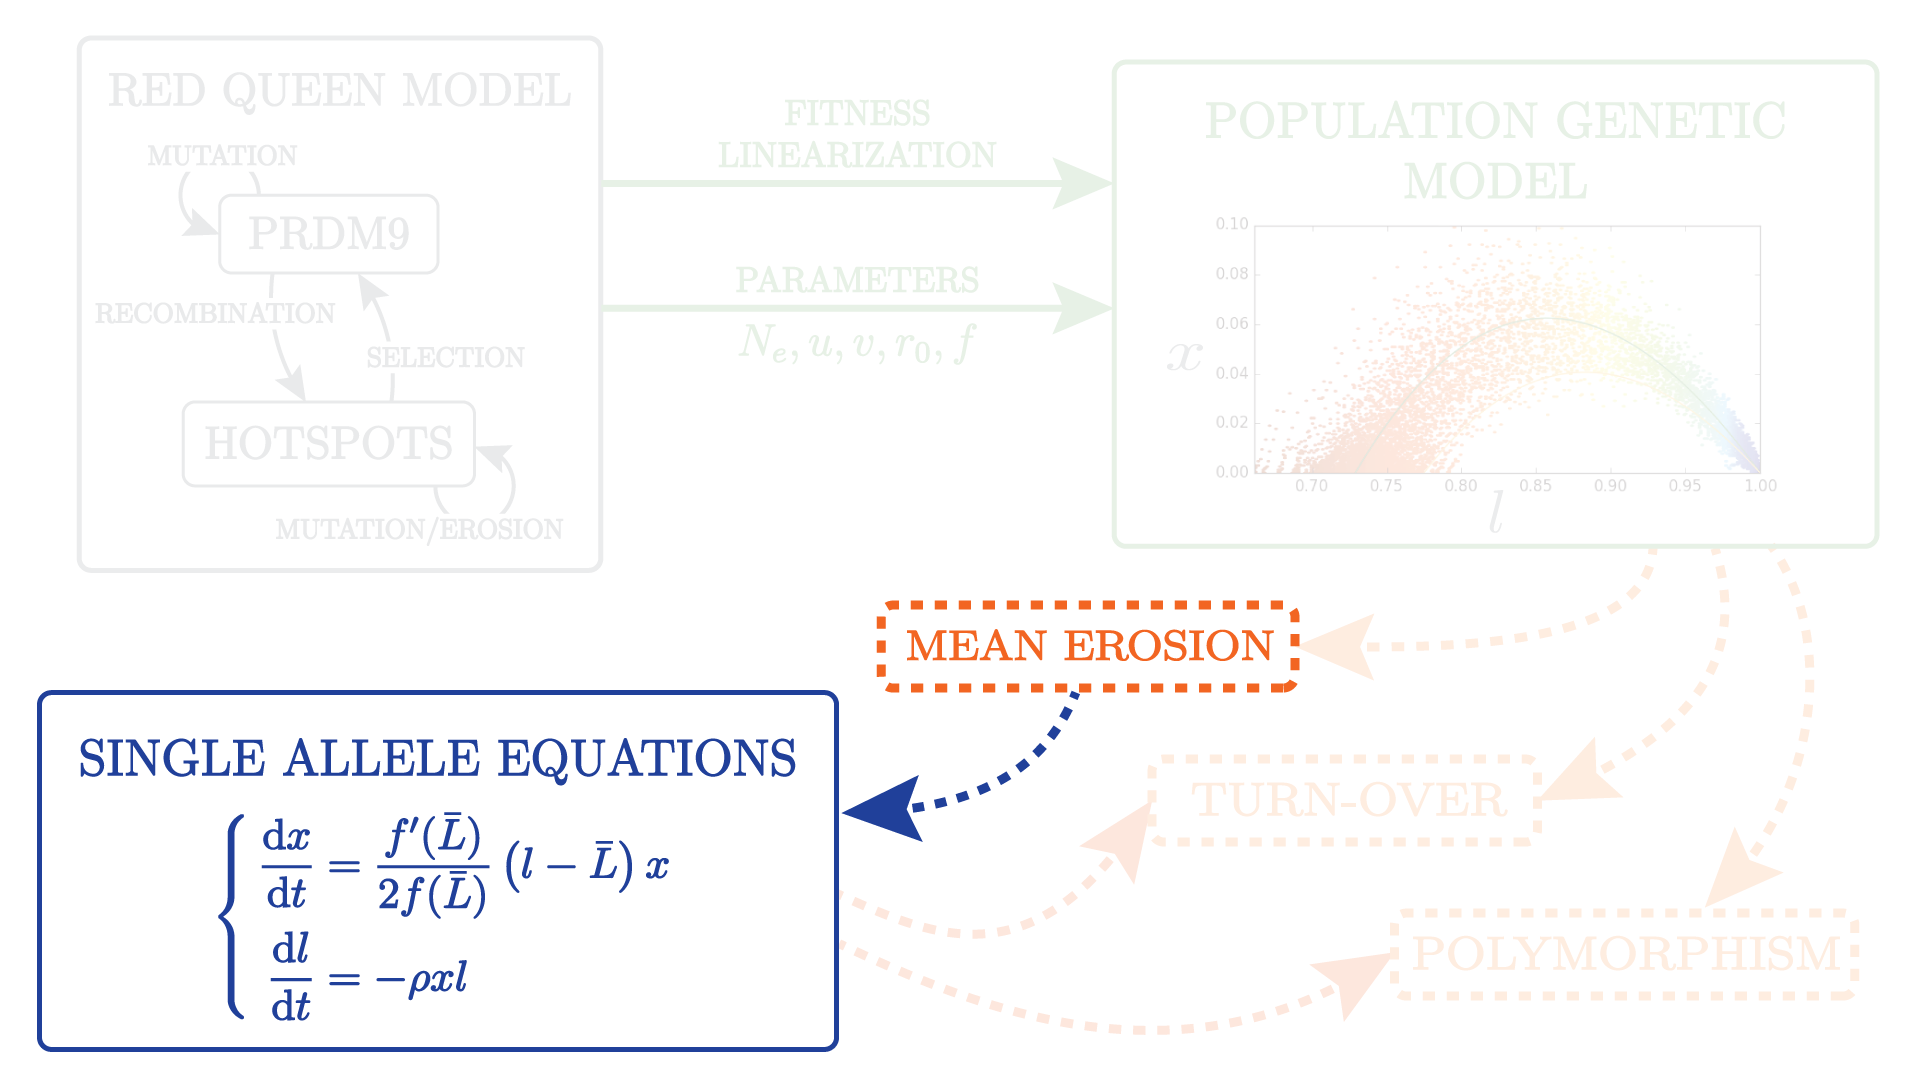
\includegraphics[width=8.5cm]{Images/overline-4.png}
	\end{center}
\end{frame}

\begin{frame}
	\begin{center}
		\Large
    	Equation for all variants in the population.
	\end{center}
	\begin{enumerate}
	\item $\forall i \in \{ 1, \, \dots, \, K \} $, $K$ is the number of variants in the population.
		
	\item $x_i$ is the frequency of the $i^{th}$ PRDM9 variant.\\
	
	\item $l_i$ is the proportion of hot hotspots associated to the $i^{th}$ PRDM9 variant.\\
		
	\item Assume there is no drift. 
	
	\item Linearise the fitness function around the mean erosion $\bar{L} = \sum_i l_i x_i$.
	\end{enumerate}
\[
  \left\{
      \begin{aligned}
          \dfrac{\mathrm{d}x_i}{\mathrm{d}t} &= \dfrac{f'(\overline{L})}{2 f(\overline{L})} \left( l_i - \overline{L} \right) x_i \\
        \dfrac{\mathrm{d}l_i}{\mathrm{d}t} &= 
        - \rho x_i l_i \\
      \end{aligned}
    \right.
\]
\end{frame}

\begin{frame}
	\begin{center}
		\Large
    	Equation for a single variant.
	\end{center}
	\begin{enumerate}
		\item Also, assume $ u N_e \gg 1$, thus $\bar{L}$ is considered fixed and an external parameter.
	\end{enumerate}
	\begin{center}
       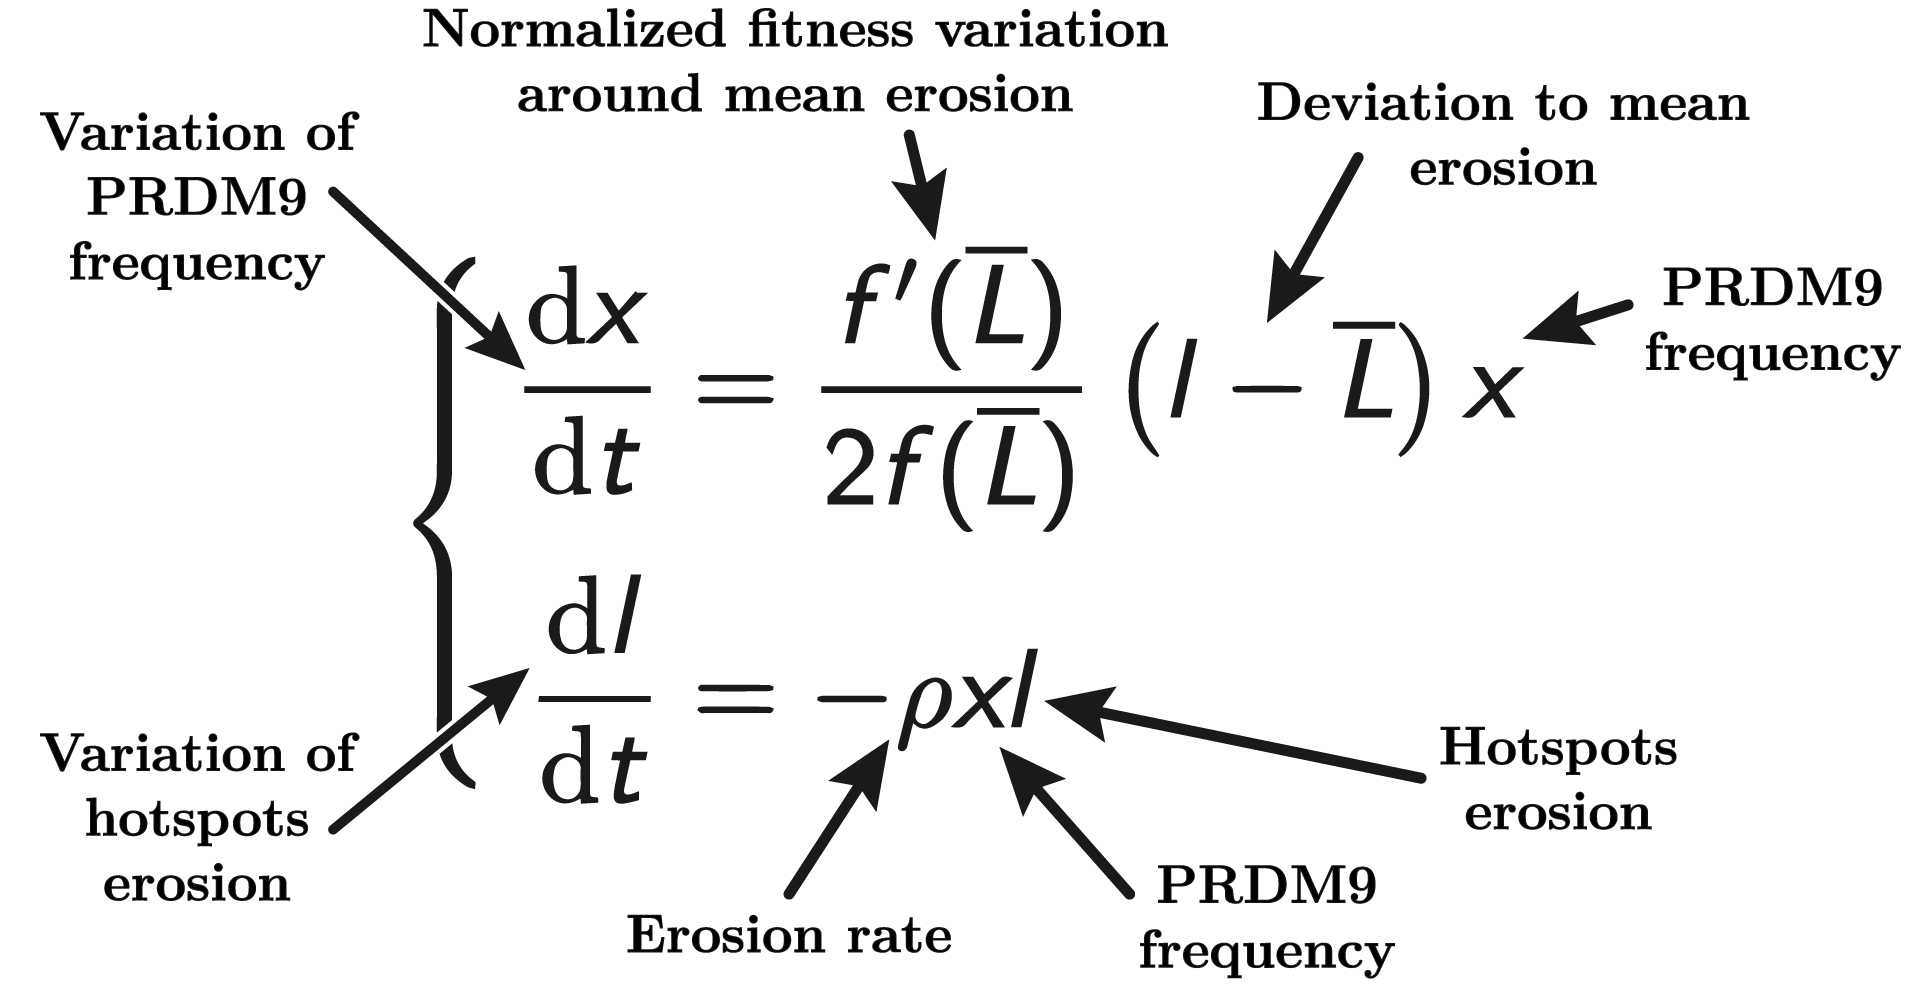
\includegraphics[width=7.5cm]{Images/equation.png}
	\end{center}
\end{frame}

\begin{frame}
\frametitle{Single allele equations}
	\begin{center}
       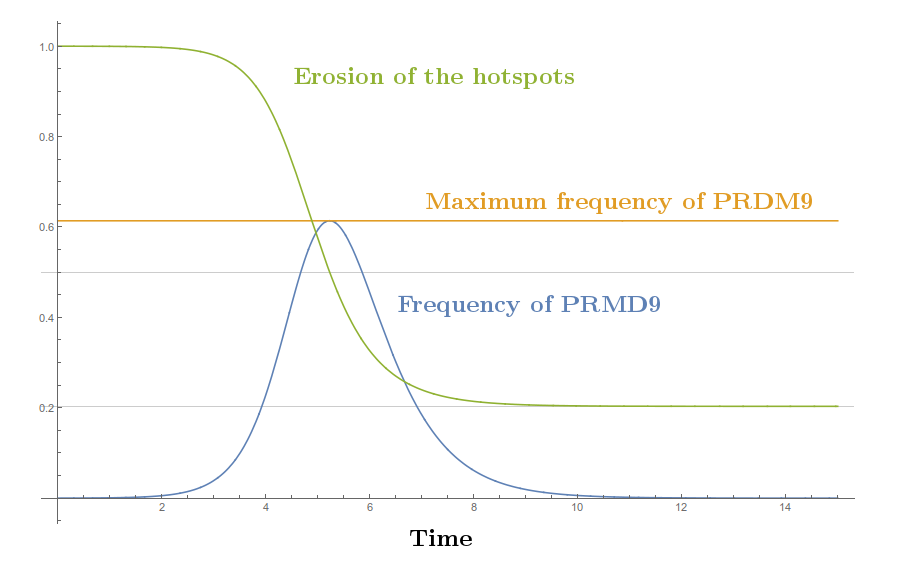
\includegraphics[width=8cm]{Images/single-allele-differential.png}
	\end{center}
\end{frame}

\begin{frame}
	\begin{center}
		\Large
    	fraction of hot hotspots as an internal clock.
	\end{center}
\[
  \left\{
      \begin{aligned}
          x(l) &=\dfrac{f'(\overline{L})}{2 \rho f(\overline{L})} (1-l + \overline{L} \mathrm{log}(l)) + x_{\mathrm{initial}} \\
           x(l_{\infty}) & \simeq  1-l_{\infty} + \overline{L} \mathrm{log}(l_{\infty}) = 0  \\
      \end{aligned}
    \right.
\]
		$\bullet$ $\rho$ is the scaled erosion rate ($u N_e r_0$). \\
		$\bullet$ $\bar{L}$ is the mean erosion. \\
		$\bullet$ $f$ is the fitness function. \\
\end{frame}

\begin{frame}
\frametitle{Single allele equations}
	\begin{center}
       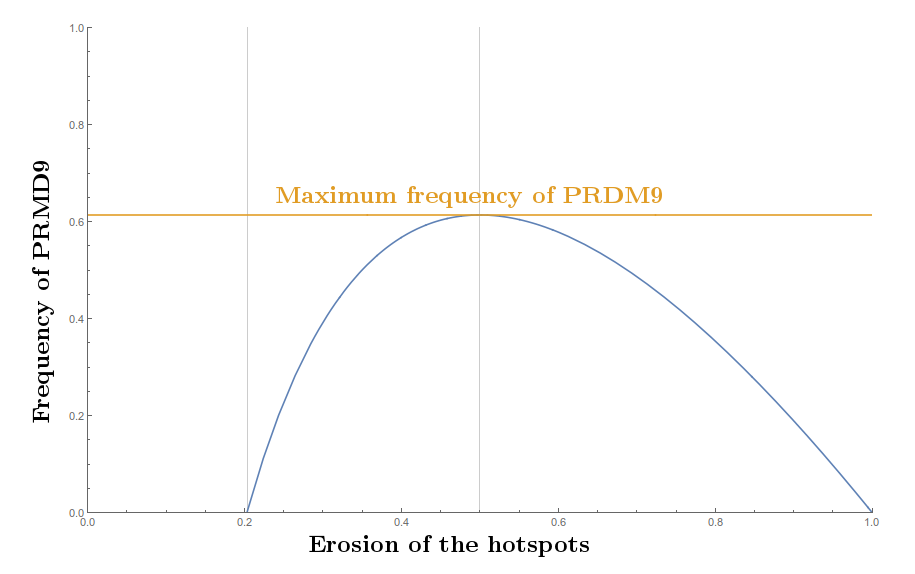
\includegraphics[width=8cm]{Images/single-allele.png}
	\end{center}
\end{frame}

\begin{frame}
	\frametitle{Comparison to simulations}
	\begin{center}
       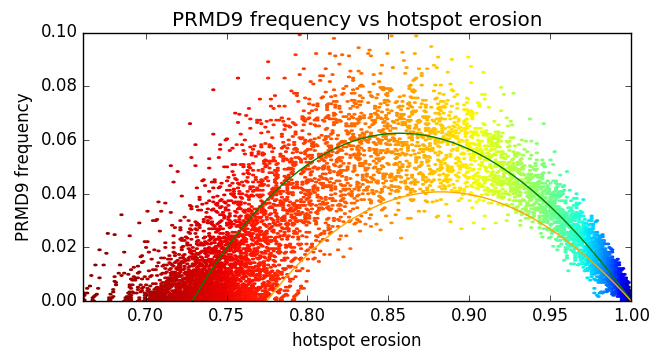
\includegraphics[width=9cm]{Images/results.png}
	\end{center}
\end{frame}

\begin{frame}
	\begin{center}
		\Large
    Polymorphism from single allele equations.
	\end{center}
\[
  K_e = \left( \sum_i x_i^2  \right)^{-1} \simeq 
  \dfrac{4 \rho f(\overline{L})}{f'(\overline{L})\left[ 1 + l_{\infty} - 2 \overline{L}  \right]}
\]
\end{frame}

\begin{frame}
	\begin{center}
		\Large
    Turn-over rate from single allele equations.
	\end{center}
\[
  \tau \sim \dfrac{2 f'(\overline{L})}{f(\overline{L})[\overline{L}-1 + \overline{L} \mathrm{log}(\overline{L})]}
\]
\end{frame}

\begin{frame}
	\begin{center}
		\Large
    Comparison of simulated data with estimated from single equation using parameters and mean erosion.
	\end{center}
\end{frame}

\begin{frame}
	\begin{center}
		\Large
    Estimation of mean erosion from parameters.
	\end{center}
\end{frame}

\begin{frame}
	\begin{center}
		\Large
    Comparison of simulated data with estimated from single equations, using only parameters.
	\end{center}
\end{frame}

\end{document}


